%\newsection{Kapitel1}

%Hier den Inhalt mit \input einfügen und die folgenden Zeilen entfernen

%\include{nomenclature.tex}

%Beginn Inhalt
%Einbeziehung der Nomenklatur, Abkürzungs- und Symbolverzeichnis
\begin{frame}
	\fta{Einleitung}

	\s{
		Während die Berechnungen von Serienschaltungen ohne parallele geschaltete 
		Bestandteile recht aufwendungsarm zu bewerkstelligen sind, wird die Analyse von 
		Gleichstromnetzwerken mit Knoten, welche n Abzweigungen aufweisen, wobei die
		Anzahl der Zweige dabei $n \geq 2$ ist, bei steigender Knotenanzahl schnell 
		unübersichtlich. Eine vielschichtige Betrachtung des Gleichstromnetzwerkes ist 
		hier von Nöten. Für die Berechnung von Gleichstromnetzwerken stehen die 
		folgenden Methoden zur Verfügung: 
		}

	\b{
		In dem Modul 'Erweiterten Gleichstromnetzwerke' werden die folgenden Inhalte
		erläutert:
		}

	\begin{itemize}
		\item Knoten- und Maschenregel
		\item Superposition
		\item Knotenpotentialanalyse
		\item Maschenstromanalyse
	\end{itemize}

	\s{
		Auch die Analyse von elektrischen Netzwerken mit mehr als einer Strom- 
		oder Spannungsquelle ist nicht trivial. Die Bestimmung aller Ströme und 
		Spannungen des elektrischen Netzwerkes aus Abbildung \ref{BildEinleitungsnetzwerk} 
		ist allein durch die Berechnungen von Serienschaltungen und Parallelschaltungen nicht 
		möglich. 
		}
 
	\fu{
		\resizebox{.5\textwidth}{!}{%
		\begin{circuitikz}
    \draw (1,2) to [R=$ $,-*] (2.5,3.5)
    to [R=$ $,-*] (4.5,3.5)
    to [R=$ $,-*] (6,2)
    to [R=$ $,-*] (6,0)
    to [R=$ $,-*] (4.5,-1.5)
    to [R=$ $,-*] (2.5,-1.5)
    to [R=$ $,-*] (1,0)
    to [R=$ $,-*] (1,2)
    (0,0) to [I=\red{$ $}] (0,2)
    (0,2) to [short] (1,2)
    (0,0) to [short] (1,0)
    (4.5,0) to [I=\red{$ $}] (4.5,2)
    (4.5,0) to [short] (6,0)
    (4.5,2) to [short] (4.5,3.5)
    (2.5,3.5) to [R=$ $] (2.5,1)
    (2.5,1) to [V={$ $}] (2.5,-1.5)
    (6,2) to [short] (7,2)
    to [R=$ $] (7,0)
    to [V={$ $}] (7,-1.5)
    to [short] (4.5,-1.5);
\end{circuitikz}%
		}
	}{{\bf Beispielnetzwerk.} Elektrisches Gleichstromnetzwerk mit einer Vielzahl an Widerständen,
	Stromquellen und Spannungsquellen. \label{BildEinleitungsnetzwerk}}
\end{frame}
%Zeigerdiagramme


\newvideofile{Komplx}{Komplexe Zahlen}

\begin{frame}
    \fta{Grundlagen Komplexe Zahlen}

     
    \s{
        Die in der Wechselstromtechnik genutzen Zeigerdiagramme geben einen schnellen Überblich über die Größe und
        die Ausrichtung der Spannung und des Stromes. Die zugrunde liegenden Begriffe der komplexen Zahlenebene und
        der Aufbau von Zeigerdiagrammen wird folgend weiter Erläutert und an einem Beispiel erklärt.
    }



    \begin{Lernziele}{Komplexe Zahlen}
        Die Studierenden können
        \begin{itemize}
            \item mit Zahlen in der komplexen Ebene umgehen.
            \item Zeigerdiagramme von komplexen Zahlen darstellen.
            \item komplexe Zahlen berechnen.
        \end{itemize}
    \end{Lernziele}

    \speech{KomplxLrnz}{1}{Das Themengebiet der komplexen Zahlen ist notwendig, 
    um tiefer in die Gegebenheiten der Wechselstromlehre und ihrer periodischen Größen einzutauchen.
    Hierzu sollen in diesem Kapitel die Grundlagen der Komplexen Zahlen vermittelt werden.
    Anschließend soll mit Zahlen in der komplexen Ebene umgegangen,
    Zeigerdiagramme von komplexen Zahlen dargestellt 
    und komplexe Zahlen berechnet werden können.} 
\end{frame}

\begin{frame}
    \ftb{Komplexe Zahlenebene}

    \s{
        Um den Aufbau von Zeigerdiagrammen zu Überblicken ist ein grundlegendes Verständnis über die komplexe 
        Zahlenebene nötig. Für die elementaren Rechenoperationen reichen die natürlichen Zahlen mit Null und die 
        rationalen Zahlen aus. Die rationalen Zahlen können als endliche oder periodische Dezimalzahlen dargestellt 
        werden. Die irrationalen Zahlen lassen sich hingegen als Dezimalzahlen darstellen, welche unendliche viele
        Stellen aufweisen und dabei nicht periodisch sind. Die reellen Zahlen setzen sich aus den rationalen Zahlen
        und den irrationalen Zahlen zusammen. Allerdings ist beispielsweise das Wurzelziehen aus einer negativen Zahl 
        in der reellen Zahlenebene nicht möglich. Hierfür wird die komplexe Zahlenebene eingeführt. in der komplexen 
        Zahlenebene wird der Raum der reellen Zahlen um die imaginäre Einheit j erweitert. So ergibt in der komplexen
        Zahlenebene das Wurzelziehen aus -1 die imaginäre Einheit j. 
    }

    \b{
        In der komplexen Zahlenebene wird die imaginäre Einheit j eingeführt, um mit komplexen Zahlen zu rechnen.
    }


    
    \begin{eq}
        \mathrm{j}=\sqrt{-1} 
    \end{eq}

    \onslide<2->{

        Das Quadrieren der imaginären Einheit ergibt wiederum -1. 
    
    \begin{eq}
        \mathrm{j}^2=-1
    \end{eq}}

    \speech{KomplxImag}{1}{In der Mathematik besteht das Problem, das die Wurzel aus einer negativen Zahl im reellen Zahlenraum nicht weiter definiert ist.
    Hier wird in der Elektrotechnik die Imaginäre Einheit jot eingeführt, welche in anderen Themenbereichen auch I genannt wird.} 
    \speech{KomplxImag}{2}{Die Definition der angegebenen Gleichung, das jot zum Quadrat gleich minus eins ergibt, ermöglicht das Radizieren von negativen Zahlen.}
\end{frame}


\begin{frame}
    \ftx{Darstellung von komplexen Zahlen}

    \s{
        Eine komplexe Zahl \underline{Z} beschreibt einen Ort in der komplexen Ebene. Um in einem zweidimensionalen
        Koordinatensystem einen Ort eindeutig festzulegen werden zwei Koordinaten benötigt. Die beiden Koordinaten zur 
        Beschreibung einer komplexen Zahl \underline{Z} werden in der komplexen Ebene als Realteil und Imaginärteil 
        beschrieben (vgl. Gleichung \ref{GleichungKomplexeZahlen}). Komplexe Zahlen werden meist durch einen Unterstrich 
        gekennzeichnet, wobei der Realteil und der Imaginärteil reelle Zahlen darstellen. 
    }

    \b{
        Kartesische Koordinaten mit dem Realteil und dem Podukt aus imaginärer Einheit und Imaginärteil:
    }

    \begin{eq}
        \underline{Z}=Realteil+\mathrm{j} \cdot Imagin"arteil  \label{GleichungKomplexeZahlen}
    \end{eq}

    \onslide<2->{
    \b{
        Der Realteil wird mit $\Re$ und der Imaginärteil mit $\Im$ abgekürzt:
    }

    \begin{eq}
        \underline{Z}=\Re(\underline{Z})+\mathrm{j} \cdot \Im(\underline{Z})  
    \end{eq}}

    \speech{KomplxDarst}{1}{Der skalare reelle Zahlenbereich wird um den Bereich der komplexen Zahlen erweitert und führt so zur komplexen Zahlenebene.
    Hier kann die komplexe Zahl beispielsweise mit kartesischen Koordinaten beschrieben werden. Die komplexe Zahl Zett unterteilt sich in den Realteil,
    gepaart mit der imaginären Einheit und dem Imaginärteil. Die Komplexen Zahlen werden mit einem Unterstrich gekennzeichnet.}
    \speech{KomplxDarst}{2}{Abgekürzt wird der Realteil Er Ee. Gelesen: Realteil von Zett. Der Imaginärteil wird mit I emm abgekürzt.}
\end{frame}


\begin{frame}
    \ftx{Darstellung von komplexen Zahlen}

    \s{
        In der Komplexene Ebene wird der Realteil auf die Abszisse und der Imaginärteil auf die Ordinate aufgetragen. 
        Es werden die Abkürzungen Re = Realteil und Im = Imaginärteil verwendet. Das Koordinatensystem einer komplexen 
        Ebene wird in der Abbildung \ref{BildKomplexeEbene} erläutert. Der Ort der komplexen Zahl kann durch 
        Richtungspfeile, welche auch als Vektoren oder Zeiger bezeichnet werden, dargestellt werden. Die Darstellung
        der komplexen Zahl in kartesischen Koordinaten erfolgt durch die Zerlegung in Realteil der komplexen Zahl 
        Re(\underline{Z}) und Imaginärteil der komplexen Zahl Im(\underline{Z}) kombiniert mit der imaginären Einheit j. 
        Komplexe Zahlen können auch in Polar-Koordinaten dargestellt werden. Dies erfolgt durch den Betrag $|\underline{Z}|$
        der komplexen Zahl \underline{Z} und durch den Winkel $\varphi$, den der Zeiger der komplexen Zahl mit der reellen Achse 
        einschließt. 
    }

    \b{
        Verwendung der komplexenen Ebene:
        \begin{itemize}
            \item<1-> Der Realteil $\Re$ wird auf der vertikalen und der Imaginärteil $\Im$ auf der horizontalen Achse aufgetragen
            \item<2-> Kartesische Koordinaten: $\Re(\underline{Z}) + \mathrm{j} \cdot \Im(\underline{Z})$
            \item<3-> Polar-Koordinaten: $|\underline{Z}| \cdot e^{j \cdot \varphi_\mathrm{Z}}  $
        \end{itemize}
    }

    \fu{
        \begin{tikzpicture}
    \draw (0,0) coordinate (K);
    \draw[very thin,color=gray] (-0.1,-0.1) grid (4.2,3.1);
    \draw[->] (-0.2,0) -- (4.4,0) node[right] {$\Re$};
    \draw[->] (0,-0.1) -- (0,3.2) node[above] {$\Im$};
    \pause
    \draw[->, color=blue] (0,0.02) -- (3,0.02) coordinate (R);
    \draw[color = blue] (3,0)node[below]	 {$\Re(\underline{Z})$};
    \draw[->, color=red] (3,0.02) -- (3,2.02) coordinate (Z);
    \draw[color = red] (3,1)node[right]	 {$\Im(\underline{Z})$};
    \draw[->] (0,0.02) -- (3,2.02);
    \draw(2.3,1.9) node	 {$\underline{Z}$};
    \pause

    %Winkel
    \draw pic[draw, angle radius = 1.2cm, <-] {angle = R--K--Z};
    \draw(1.4,0.5) node{$\varphi_\mathrm{Z}$};
    \draw(1,1)node {$|\underline{Z}|$};
\end{tikzpicture}
    }{{\bf Zeigerdiagramm einer komplexen Zahl.} Eine komplexe Zahl $\underline{Z}$, welche sich durch $Re(\underline{Z})$ und $Im(\underline{Z})$
    in kartesischen Koordinaten und durch den Betrag der komplexen Zahl $|\underline{Z}|$ sowie den zugehörigen Winkel
    $\varphi$ in Polar-Kooradinaten darstellen lässt. \label{BildKomplexeEbene}}

    \speech{KomplxDarstEbn}{1}{Folgend wird die komplexe Ebene dargestellt. Hier wird der Realteil auf der Abszisse und der Imaginärteil auf der Ordinate aufgetragen.}
    \speech{KomplxDarstEbn}{2}{Eine komplexe Zahl Zett kann in der komplexen Ebene dargestellt werden. Nach der zuvor getroffenen Definition, 
    kann die komplexe Zahl in den Realteil von Zett und den Imaginärteil von Zett unterteilt werden.}
    \speech{KomplxDarstEbn}{3}{Außerdem kann eine komplexe Zahl auch in Polarkoordinaten dargestellt werden.
    Hierbei wird der Betrag der komplexen Zahl und der Winkel Vieh zur Abszisse als Definition verwendet.}
\end{frame}


\begin{frame}
    \ftx{Koordinatentransformation}

    \s{
        Die beiden Darstellungsformen lassen sich ineinander transformieren. Behilflich ist hier die Euler'sche Formel. 
        Die Euler'sche Formel zeigt, dass sich der Ordinatenwert und der Abszissenwert des Einheitskreises
        durch die trigonometrischen Funktionen Kosinus und Sinus berechnen lassen. Die Euler'sche Formel wird in der Gleichung 
        \ref{GleichungEuler} dargestellt. 

        \begin{eq}
            \mathrm{e}^{\mathrm{j} \cdot \chi} = \cos(\chi) + \mathrm{j} \cdot \sin(\chi)    \label{GleichungEuler}
        \end{eq}
    
        Unter Verwendung der Euler'schen Formel können durch die Hinzunahme des Betrages der komplexen Zahl die Polar-Koordinaten
        in kartesische Koordinaten transformiert werden. Dies wird durch die Gleichung \ref{GleichungKartesisch} erläutert. 
    
        \begin{eq}
            \underline{Z} = |\underline{Z}| \cdot \cos(\varphi) + \mathrm{j} \cdot |\underline{Z}| \cdot \sin(\varphi) = \Re(\underline{Z}) + \mathrm{j} \cdot \Im(\underline{Z}) \label{GleichungKartesisch}
        \end{eq}
    
        Über den Satz des Pythagoras lässt sich aus den bekannten Realteil und Imaginärteil der Betrag der komplexen Zahl
        für die Polar-Koordianten bestimmen. Der dazugehörige Winkel ergibt sich aus dem arctan mit dem Verhältnis aus Imaginärteil
        zu Realteil im Argument. Mit diesen Informationen kann eine komplexe Zahl wie in der Gleichung \ref{GleichungPolar} 
        in Polar-Koordinaten transformiert werden. 
    
        \begin{eq}
            \underline{Z} = \sqrt{(\Re(\underline{Z}))^2+(\Im(\underline{Z}))^2} \cdot \mathrm{e}^{\mathrm{j} \cdot \arctan(\frac{\Im(\underline{Z})}{\Re(\underline{Z})}) } = |\underline{Z}| \cdot \mathrm{e}^{\mathrm{j} \cdot \varphi} \label{GleichungPolar}
        \end{eq}
    }

    \b{
        \begin{itemize}
            \item Euler'sche Formel: 
            \begin{eq}
                \mathrm{e}^{\mathrm{j} \cdot \chi} = \cos(\chi) + \mathrm{j} \cdot \sin(\chi)  
            \end{eq}
            \item Kartesische Koordianten:
            \begin{eq}
                \underline{Z} = |\underline{Z}| \cdot \cos(\varphi) + \mathrm{j} \cdot |\underline{Z}| \cdot \sin(\varphi) = \Re(\underline{Z}) + \mathrm{j} \cdot \Im(\underline{Z}) 
            \end{eq}
            \item Polar-Koordinaten:
            \begin{eq}
                \underline{Z} = \sqrt{(\Re(\underline{Z}))^2+(\Im(\underline{Z}))^2} \cdot \mathrm{e}^{\mathrm{j} \cdot \arctan(\frac{\Im(\underline{Z})}{\Re(\underline{Z})}) } = |\underline{Z}| \cdot e^{j \cdot \varphi} 
            \end{eq}
        \end{itemize}
    }

    \speech{KomplxKoordtr}{1}{Über die Eulersche Formel können Winkelangaben, in die Bestandteile der Kartesischen Koordinaten aufgeteilt werden.
    Um die komplexe Zahl aus den Polarkoordinaten in die kartesischen Koordinaten zu überführen, 
    wird über die Eulersche Formel mit dem Betrag und dem Winkel der komplexen Zahl der Realteil und der Imaghinärteil bestimmt.
    Andersherum lässt sichd er Betrag der komplexen Zahl über den Satz des Pütagoras bestimmen. Der Winkel ergibt sich aus der Arcustangensfunktion.}
\end{frame}


\begin{frame}
    \ftx{Darstellungsformen komplexer Zahlen}

    \begin{Merksatz}{Darstellungsformen komplexer Zahlen}
        Kartesische Darstellung:
        \begin{eq}
            \underline{Z} = \Re(\underline{Z}) + j \cdot \Im(\underline{Z}) \nonumber
        \end{eq}
        Polarform:
        \begin{eq}
            \underline{Z} = |\underline{Z}| \cdot e^{j \cdot \varphi}   \nonumber
        \end{eq}
        Trigonometrische Darstellung:
        \begin{eq}
            \underline{Z} = |\underline{Z}| (\cos(\varphi) + j \cdot \sin(\varphi))   \nonumber
        \end{eq}
    \end{Merksatz}

    \speech{KomplxMrk1}{1}{Komplexe Zahlen lassen sich über den Realteil und Imaginärteil in Kartesischen Koordinaten,
    über die Polarform mit dem Betrag und dem zugehörigen Winkel,
    sowie mit den Trigonometrischen Funktionen darstellen und ineinander umrechnen.}
\end{frame}

\begin{frame}
    \ftx{Grundrechenarten und Operationen}

    \s{
        Zu den Operationen bei komplexen Zahlen zählt die Konjugation. Beim Konjugieren einer komplexen Zahl wird der 
        j durch -j ersetzt (Negation des Imaginärteils). Die Konjugation wird wie in Gleichung \ref{GleichungKonj} dargestellt mit einem
        Stern gekennzeichnet. 
    }

    \b{
        Konjugation:
    }

    \begin{eq}
        \underline{Z}^* = (\Re(\underline{Z}) + \mathrm{j} \cdot \Im(\underline{Z}))^*= \Re(\underline{Z}) - \mathrm{j} \cdot \Im(\underline{Z})   \label{GleichungKonj}
    \end{eq}

    \s{
        Der Betrag einer komplexen Zahl lässt sich durch die Multiplikation der komplexen Zahl mit ihrer Konjugierten
        bestimmen (vgl. Gleichung \ref{GleichungBetrag}). Statt des Betrages, welcher eine Wurzel enthält, wird auch das Betragsquadrat 
        verwendet. Es stellt ebenfalls ein Maß für den Abstand der Zahl zum Ursprung dar, ist aber einfacher zu berechnen.
    }

    \onslide<2->{
    \b{
        Betrag und Betragsquadtrat
    }

    \begin{eq}
        |\underline{Z}| = \sqrt{\underline{Z} \cdot \underline{Z}^*} \rightarrow |\underline{Z}|^2 = \underline{Z} \cdot \underline{Z}^*        \label{GleichungBetrag}
    \end{eq}}

    \speech{KomplxOperat}{1}{Bei der sogennanten Konjugiert-Komplexen Darstellung einer Zahl handelt es sich um eine komplexe Zahl, 
    bei welcher das Vorzeichen des Imaginärteiles negiert wird. So wird beispielsweise aus dem positiven Imaginärteil ein negativer.}
    \speech{KomplxOperat}{2}{Das Betragsquadrat quadriert den Betrag einer Komplexen Zahl. 
    Es wird ebenso wie der normale Betrag einer komplexen Zahl als Maß für den Abstand zum Ursprung verwendet. }
\end{frame}

\begin{frame}
    \ftx{Grundrechenarten und Operationen}
    \s{
        Bei der Addition und der Subtraktion von komplexen Zahlen empfiehlt es sich, diese zunächst in kartesiche 
        Koordianten umzuwandeln. Auf diese Weise lassen sich der Realteil und der Imaginärteil der komplexen Zahl
        separat miteinander verrechnen. 
    }
    \b{
        Addition und Subtraktion:
    }
    \begin{eqa}
        \underline{Z}_1+\underline{Z}_2 = \Re(\underline{Z}_1) + \Re(\underline{Z}_2) +j \cdot (\Im(\underline{Z}_1) + \Im(\underline{Z}_2)) \\
        \underline{Z}_1-\underline{Z}_2 = \Re(\underline{Z}_1) - \Re(\underline{Z}_2) -j \cdot (\Im(\underline{Z}_1) - \Im(\underline{Z}_2))
    \end{eqa}

    \s{
        Die Darstellung in Polar-Koordinaten empfiehlt sich für die Verrechnungen von komplexen Zahlen durch Multiplikation
        und Division. Die Multiplikation von komplexen Zahlen setzt sich auf dem Produkt der Beträge und der Summe der jeweiligen
        Winkel zusammen (vgl. Gleichung \ref{GleichungMultiplikation}). Bei der Division werden die Beträge dividiert und die Winkel 
        voneinander subtrahiert (vgl. Gleichung \ref{GleichungDivision}). 
    }

    \onslide<2->{
    \b{
        Multiplikation und Division:
    }

    \begin{eq}
        \underline{Z}_1 \cdot \underline{Z}_2 = |\underline{Z}_1| \cdot |\underline{Z}_2| \cdot e^{j \cdot (\varphi_1+\varphi_2)} \label{GleichungMultiplikation}
    \end{eq}

    \begin{eq}
        \frac{\underline{Z}_1}{\underline{Z}_2} = \frac{|\underline{Z}_1|}{|\underline{Z}_2|} \cdot e^{j \cdot (\varphi_1-\varphi_2)} \label{GleichungDivision}
    \end{eq}}

    \speech{KomplxGrundrech}{1}{Grundsätzlich wird bei verschiedenen komplexen Zahlen gerechnet wie mit unterschiedlichen Variablen. 
    Bei der Addition werden die Realteile und imaginärteile jeweils seperat addiert.
    Ebenso verhält es sich bei der Subtraktion, auch hier werden die Realteile und Imaginärteile jeweils für sich voneinander subtrahiert.}
    \speech{KomplxGrundrech}{2}{Bei der Multiplikation wird der Betrag der Komplexen Zahlen miteinander Multipliziert und die Winkel im Exponenten addiert.
    Die Division von komplexen Zahlen erfolgt durch die Division der Beträge und der Subtraktion der Winkel.}
\end{frame}


\begin{frame}
    \ftx{Grundrechenarten komplexer Zahlen}

    \begin{Merksatz}{Grundrechenarten komplexer Zahlen}
        Für die {\bf Addition und Subtraktion} wird in der Regel die {\bf kartesische Darstellungsform} für komplexen Zahlen verwendet.
        Bei der {\bf Multiplikation und Division} von komplexen Zahlen wird die {\bf Polarform} gewählt. 
    \end{Merksatz}

    \speech{KomplxMrk2}{1}{Für die Addition und die Subtraktion wird in der Regel die kartesische Darstellungsform für komplexen Zahlen verwendet.
    Bei der Multiplikation und der Division von komplexen Zahlen wird die Polarform zur Berechnung gewählt.}
\end{frame}


\begin{frame}
    \ftx{Grundrechenarten und Operationen}
    \s{
        Da die Division zunächst nur für reelle Zahlen außer Null definiert ist, wird die komplexe Zahl im Nenner so erweitert, dass 
        dieser reell wird.
    }
    \b{
        Division durch konjugiert komplexe Erweiterung:
    }
    \begin{eq}
        \frac{\underline{Z}_1}{\underline{Z}_2} = \frac{\underline{Z}_1}{\underline{Z}_2} \cdot \frac{\underline{Z}_2^*}{\underline{Z}_2^*} = \frac{\underline{Z}_1 \cdot \underline{Z}_2^*}{|\underline{Z}_2|^*} 
    \end{eq}

    \s{
        Durch die Addition einer komplexen Zahl mit ihrer konjugiert komplexen hebt sich ihr Imaginärteil auf (vgl. Gleichung \ref{GleichungRealteil}). 
        Entsprechend verschwindet durch die Subtraktion der Realteil (vgl. Gleichung \ref{GleichungImaginärteil}).
    }

    \onslide<2->{
    \b{
        Realteil und Imaginärteil berechnen:
    }
    \begin{eq}
        \Re(\underline{Z}) = \frac{\underline{Z}+\underline{Z}^*}{2} \label{GleichungRealteil}
    \end{eq}
    \begin{eq}    
        \Im(\underline{Z}) = \frac{\underline{Z}-\underline{Z}^*}{2j} \label{GleichungImaginärteil}
    \end{eq}}

    \speech{KomplxWeitere}{1}{Die Division von komplexen Zahlen kann auch durch die konjugiert-komplexe Erweiterung erfolgen.} 
    \speech{KomplxWeitere}{2}{Durch die Addition einer komplexen Zahl mit ihrer konjugiert komplexen hebt sich ihr Imaginärteil auf. 
    Entsprechend verschwindet durch die Subtraktion der Realteil.
    Je nach Anwendungsfall können mit diesen Operationen die Rechnungen vereinfacht werden.}     
\end{frame}


\begin{frame}
    \ftb{Graphische Darstellung und Rechnungen mit komplexen Zahlen}

    \s{
        Mithilfe von Zeigerdiagrammen lassen sich komplexe Zahlen auch zeichnerisch lösen. Werden die komplexen
        Zahlen wie empfohlen in der kartesischen Form dargestellt, können die Bestandteile der Realteile und der 
        Imaginärteile direkt abgelesen werden und in ein Koordinatensystem eingestragen werden. Die komplexen Zahlen 
        werden beispielsweise in der Abbildung \ref{BildKomplexRechnung} eingetragenen. Bei der Addition von komplexen Zahlen wird entweder
        $Z_\mathrm{1}$ an $Z_\mathrm{2}$ gesetzt oder umgekehrt. Denn bei der Addition gilt weiterhin das Kommutativgesetz. Hier werden durch 
        die gestrichelten Pfeile die Parallelverschiebungen von $Z_\mathrm{1}$ und $Z_\mathrm{2}$ angegeben. Die Verschiebungen enden beide an 
        der selben Koordinate. Hier können separat der Realteil und der Imaginärteil aus der Summe der beiden komplexen 
        Zahlen abgelesen werden. 
    }

    \b{
        Rechenoperationen im Zeigerdiagramm - Addition:

        \begin{itemize}
            \item[1.] <2-> Parallelverschiebung $Z_\mathrm{2}$ an die Spitze von $Z_\mathrm{1}$
            \item[2.] <3-> Realteil und Imaginärteil ablesen
        \end{itemize}
    }

    \fu{
        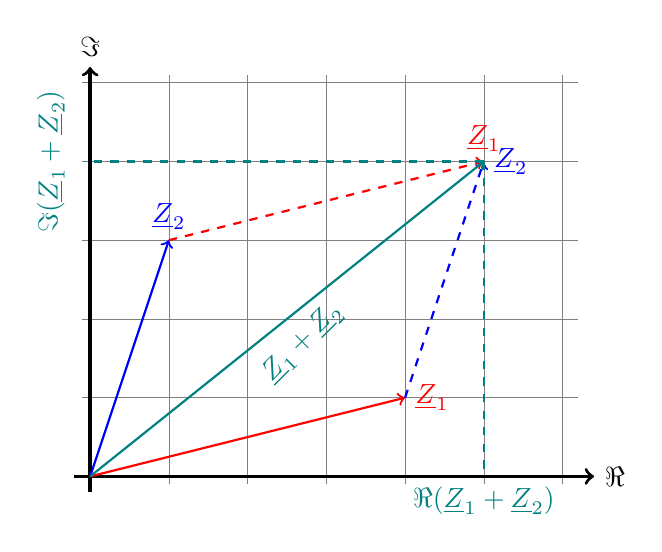
\begin{tikzpicture}
    \draw (0,0) coordinate (K);
    \draw[very thin,gray] (-0.1,-0.1) grid (6.2,5.1);
    \draw[->, very thick] (-0.2,0) -- (6.4,0) node[right] {$\Re$};
    \draw[->, very thick] (0,-0.2) -- (0,5.2) node[above] {$\Im$};
    \draw[->, thick, red] (0,0) -- (4,1) node[right] {$\underline{Z}_\mathrm{1}$};
    \draw[->, thick, blue] (0,0) -- (1,3) node[above] {$\underline{Z}_\mathrm{2}$};
    \pause

    \draw[->, dashed, thick, blue] (4,1) -- (5,4) node[right] {$\underline{Z}_\mathrm{2}$};
    \draw[->, dashed, thick, red] (1,3) -- (5,4) node[above] {$\underline{Z}_\mathrm{1}$};
    \pause

    \draw[->, thick, teal] (0,0) -- (5,4);
    \draw(2.7,1.7) node [teal, rotate=45] {$\underline{Z}_\mathrm{1}+\underline{Z}_\mathrm{2}$};
    \draw[dashed, thick, teal] (5,4) -- (0,4)
    (-0.5,4) node[rotate=90] {$\Im(\underline{Z}_\mathrm{1}+\underline{Z}_\mathrm{2}$)};
    \draw[dashed, thick, teal] (5,4) -- (5,0) node[below] {$\Re(\underline{Z}_\mathrm{1}+\underline{Z}_\mathrm{2}$)};
\end{tikzpicture}
    }{{\bf Addition von komplexen Zahlen.} Zeichnerische Lösung einer Addition von zwei komplexen Zahlen im Zeigerdiagramm. \label{BildKomplexRechnung}}

    \speech{KomplxGraphAdd}{1}{Gezeigt wird die Komplexe Ebene mit der Aufteilung in Realteil und Imaghinärteil.
    Außerdem werden die Zahlen Zett eins in rot und Zett zwei in blau dargestellt.
    Hier soll nun die Addition der beiden komplexen Zahlen grafisch gelöst werden.}
    \speech{KomplxGraphAdd}{2}{Dafür wird eine der Zahlen parallel an der anderen komplexen Zahl verschoben. 
    Dabei ist es nach dem Kommutativgesetz unerheblich, welche komplexe Zahl womit addiert wird.}
    \speech{KomplxGraphAdd}{3}{Nun können der Realteil und der Imaginärteil aus der Summe der beiden komplexen Zahlen abgelesen und notiert werden.}
\end{frame}


\begin{frame}
    \ftx{Zeigerdiagramme - Subtraktion}

    \s{
        Die zeichnerische Lösung der Subtraktion von komplexen Zahlen erfolgt vergleichbar mit der Addition. 
        Zu beachten ist dabei, dass wie in anderen Zahlensystemen bei der Subtraktion von zwei komplexen Zahlen
        das Kommutativgesetz nicht gilt. Wird von der komplexen Zahl $Z_\mathrm{2}$ $Z_\mathrm{1}$ subtrahiert, ändert sich die Richtung
        von $Z_\mathrm{1}$. Hier erfolgt dann wieder die Parallelverschiebung, allerdings lediglich von $Z_\mathrm{1}$. An dem sich ergebenen
        neuen Vektor können dann wieder der Realteil und der Imaginärteil abgelesenw erden. 
    }

    \b{
        Rechenoperationen im Zeigerdiagramm - Subtraktion:

        \begin{itemize}
            \item[1.] <1-> Zeigerumkehr bei Negation
            \item[2.] <2-> Zeiger $Z_\mathrm{1}$ verschieben: Fußpunkt von $Z_\mathrm{1}$ zur Spitze von $Z_\mathrm{2}$
            \item[3.] <3-> Realteil und Imaginärteil ablesen
        \end{itemize}
    }

    \fu{
        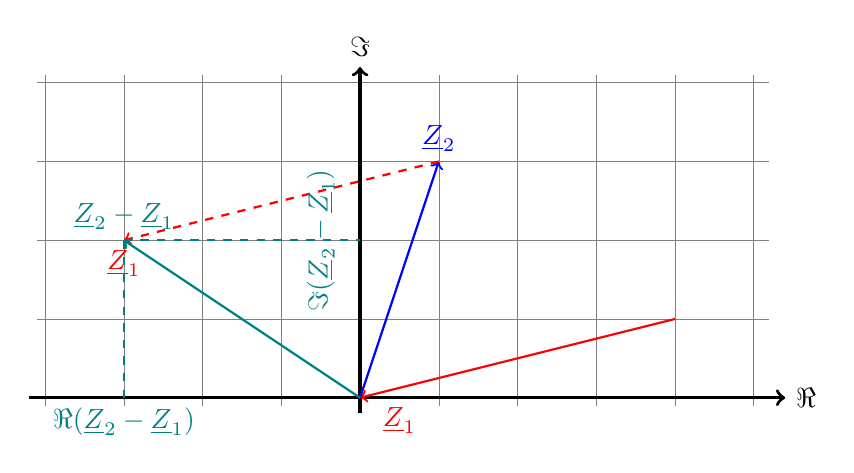
\begin{tikzpicture}
    \draw (0,0) coordinate (K);
    \draw[very thin,gray] (-4.1,-0.1) grid (5.2,4.1);
    \draw[->, very thick] (-4.2,0) -- (5.4,0) node[right] {$\Re$};
    \draw[->, very thick] (0,-0.2) -- (0,4.2) node[above] {$\Im$};
    \draw[->, thick, red] (4,1) -- (0,0);
    \draw(0.5,0) node [below,red] {$\underline{Z}_\mathrm{1}$};
    \draw[->, thick, blue] (0,0) -- (1,3) node[above] {$\underline{Z}_\mathrm{2}$};
    \pause

    \draw[->, dashed, thick, red] (1,3) -- (-3,2) node[left, below] {$\underline{Z}_\mathrm{1}$};
    \pause

    \draw[->, thick, teal] (0,0) -- (-3,2) node [teal, above] {$\underline{Z}_\mathrm{2}-\underline{Z}_\mathrm{1}$};
    \draw[dashed, thick, teal] (-3,2) -- (0,2)
    (-0.5,2) node[rotate=90] {$\Im(\underline{Z}_\mathrm{2}-\underline{Z}_\mathrm{1}$)};
    \draw[dashed, thick, teal] (-3,2) -- (-3,0) node[below] {$\Re(\underline{Z}_\mathrm{2}-\underline{Z}_\mathrm{1}$)};
\end{tikzpicture}
    }{{\bf Subtraktion von komplexen Zahlen.} Zeichnerische Lösung einer Subtraktion von zwei komplexen Zahlen im Zeigerdiagramm.}

    \speech{KomplxGraphSub}{1}{Ähnlich wie bei der Addition wird bei der Subtraktion von komplexen Zahlen vorgegangen.
    Wieder wird die komplexe Ebene mit dem Realteil und dem Imaginärteil dargestellt.
    Nun wird aber Zett eins von Zett zwei subtrahiert. 
    Hierfür wird die Richtung des Zeigers Zett eins umgekehrt. }
    \speech{KomplxGraphSub}{2}{Anschließend wird der Zeiger von Zett eins so verschoben,
    dass das Ende von Zett eins an der Spitze von Zett zwei anliegt.}
    \speech{KomplxGraphSub}{3}{Folgend werden wieder der Realteil und der Imaginärteil aus der Differenz der beiden komplexen Zahlen abgelesen und notiert.}
\end{frame}

  
\begin{frame}
    \ftx{Zeigerdiagramme - Multiplikation}

    \s{
        Die in der Abbildung \ref{BildMultiplikation} dargestellten komplexen Zahlen $\underline{Z}_\mathrm{1}$ und $\underline{Z}_\mathrm{2}$ werden zur 
        Multiplikation in Polar-Koordinaten abgebildet. Durch die zuvor beschriebenen Rechnenregeln der Multiplikation 
        für komplexe Zahlen können die Werte für die für das Ergebnis $\underline{Z}_\mathrm{3}$ bestimmt werden. Die Multiplikation
        aus den Zeigerlängen gibt die Länge des Produktes an. Die Summe aus den beiden komplexen Zahlen den Winkel der neuen
        komplexen Zahl an. 
    }

    \b{
        Rechenoperationen im Zeigerdiagramm - Multiplikation: (Zeichnung nicht maßstabsgetreu!)

        \begin{itemize}
            \item[1.] <2-> Winkel $\varphi_\mathrm{1}+\varphi_\mathrm{2}$ berechnen und einzeichnen
            \item[2.] <3-> Länge $Z_1 \cdot Z_\mathrm{2}$ berechnen und eintragen
            \item[3.] <4-> Realteil und Imaginärteil ablesen
        \end{itemize}
    }
    
    \fu{
        \begin{tikzpicture}
    \draw (0,0) coordinate (U);
    \draw (4,0) coordinate (0);
    \draw[very thin,gray] (-3.1,-0.1) grid (5.2,4.1);
    \draw[->, very thick] (-3.2,0) -- (5.4,0) node[right] {$\Re$};
    \draw[->, very thick] (0,-0.2) -- (0,4.2) node[above] {$\Im$};
    \draw[->, thick, red] (0,0) -- (4,1) coordinate (1);
    \draw(4,1) node [right,red] {$\underline{Z}_\mathrm{1}$};
    \draw[->, thick, blue] (0,0) -- (1,3) coordinate (2);
    \draw(1,3) node [above,blue] {$\underline{Z}_\mathrm{2}$};
    \draw pic[draw,red, very thick, angle radius = 3cm, ->] {angle = 0--U--1} (3.5,0.5) node[very thick, red]{$\varphi_\mathrm{1}$};
    \draw pic[draw,blue, very thick, angle radius = 2cm, ->] {angle = 0--U--2} (1.5,1.7) node[very thick, blue]{$\varphi_\mathrm{2}$};
    \pause

    \draw (-2,4) coordinate (3);
    \draw pic[draw, teal, very thick, angle radius = 1cm, ->] {angle = 0--U--3} (-1.2,0.5) node[very thick, teal]{$\varphi_\mathrm{1}+\varphi_\mathrm{2}$};
    \pause

    \draw[->, thick, teal] (0,0) -- (-2,4);
    \pause

    \draw[dashed, thick, teal] (-2,0) -- (-2,4) node[above] {$\underline{Z}_\mathrm{2} \cdot \underline{Z}_\mathrm{1}$};
    \draw[dashed, thick, teal] (0,4) -- (-2,4);
\end{tikzpicture}
    }{{\bf Multiplikation von komplexen Zahlen.} Zeichnerische Lösung einer Multiplikation von zwei komplexen Zahlen in Polar-Koordinaten im Zeigerdiagramm. \label{BildMultiplikation}}

    \speech{KomplxGraphMulti}{1}{Bei der grafischen Multiplikation ist ein wenig Rechnen notwendig.
    Hier werden die komplexen Zahln Zett eins und Zett zwei in der komplexen Ebene in ihrer Polarform dargestellt.}
    \speech{KomplxGraphMulti}{2}{Um das Produkt aus den beiden komplexen Zahlen zu bestimmen,
    wird im ersten Schritt die Summe aus den beiden Winkel der komplexen Zahlen gebildet und notiert.}
    \speech{KomplxGraphMulti}{3}{Im zweiten Schritt werden die beiden Beträgen der komplexen Zahlen miteinander multipliziert und eingetragen.}
    \speech{KomplxGraphMulti}{4}{Abschließend kann das Ergebniss nach der Berechnung auch grafisch veranschaulicht werden.}
\end{frame} 
\newpage
%Anwendung komplexe Zahlen in der Wechselstromtechnik

\begin{frame}
    \fta{Zeigerdiagramme in der Wechselstromtechnik}
    
    \s{
        In der Wechselstromtechnik finden die komplexen Zahlen unter Anderem als Zeiger Verwendung.  
        In linearen Netzwerken haben sinusförmige und monofrequente Quellengrößen nur sinusförmige und monorfequente 
        Spannungen und Ströme zur Folge. Im Stationären Zustand unterscheiden sich die Spannungen und Ströme nur in 
        ihrer Amplitude und der zugehörigen Phase. Alle Signale haben dabei eine identische Frequenz. Die Stationären
        und harmonischen Schwingungen können durch ihren Zeitverlauf im Liniendiagramm oder durch komplexe Zahlen durch
        Zeiger dargestellt werden. Die Beschreibung von Schwingungen durch komplexe Zahlen ermöglicht die Darstellung 
        durch ruhende Zeiger, wobei nur die relative Lage zueinander ausgedrückt wird. 
    }
    
    \b{
    
    }
    
    \begin{Lernziele}{Zeigerdiagramme}
        Die Studierenden
        \begin{itemize}
            \item verstehen die Kenngrößen von periodischen Wechselspannungen.
            \item können mit den komplexen Drehzeigern der Amplituden umgehen.
        \end{itemize}
    \end{Lernziele}
    
\end{frame}

\begin{frame}
    \ftb{Periodische Wechselspannung}
    
    \s{
        In der Abbildung \ref{BildWechselspannungssignal} wird ein Wechselspannungssignal mit dem Scheitelwert (Amplitudenwert) $\hat{U}$
        dargestellt. Der Versatz des Wechselspannungssignals auf der Abszisse wird durch den Zeitpunkt $t_\mathrm{0}$
        ausgedrückt. Der Punkt in dem das Wechselspannungssignal die Ordinate kreuzt gibt den Wechselspannungswert 
        U zum Zeitpunkt t=0 an. 
        
        Das Wechselspannungssignal ist periodisch in T. Eine Periode wird bei dem angegebenen Wechselspannungsignal
        durch einen kompletten Durchlauf einer positiven und negativen Halbwelle definiert. So wird ab $t_\mathrm{0}$ nach einer 
        Periode der Zeitpunkt $t_0+T$ und nach zwei Perioden der Zeitpunkt $t_\mathrm{0+2T}$ erreicht. 
        
        Mit der Übertragung der angegebenen Werte auf ein Kreisdiagramm lässt sich der Zusammenhang der Wechselspannung 
        mit der komplexen Darstellung erklären. Auf diese Weise kann die Wechselspannungsgröße $U(t=0)$ zum Zeitpunkt 0 
        durch die Länge und Ausrichtung des Zeigers beschrieben werden. Der Scheitelwert enspricht der Länge des Zeigers
        im Kreisdiagramm. Der Winkel $\varphi_\mathrm{u}$ beschreibt den Phasenwinkel zum Zeitpunkt $t=0$. 
    }
    
    \b{
        Anwendung von komplexen Zahlen in der Wechselstromtechnik
        
        \begin{itemize}
            \item <1-> Sinusförmige und harmonische Quellengrößen, Scheitelwert $\hat{U}$ und Phasenverschiebung $t_\mathrm{0}$
            \item <2-> Periodendauer T, Wiederholung von Perioden
            \item <3-> Stationärer Zustand $\rightarrow$ Spannungen und Ströme unterscheiden sich nur in Amplitude und Phase
            \item <4-> Schwingungen können durch Zeiger dargestellt werden
        \end{itemize}
    }
    
    \fu{
        %vergrößern auf Folienbreite
        \resizebox{0.95\textwidth}{!}{
            \begin{circuitikz}[domain=-1:8.5,samples=100]
    %Gitter
    \draw[very thin,color=gray] (-1.1,-2.1) grid (8.7,2.1);
    \draw[->] (-1.2,0) -- (8.9,0) node[right] {$t$};
    \draw[->] (0,-2.1) -- (0,2.2) node[above] {};
    \draw (0,-2.1) node[below] {$0\ ms$};
    \draw (2,-2.1) node[below] {$10\ ms$};
    \draw (4,-2.1) node[below] {$20\ ms$};
    \draw (6,-2.1) node[below] {$30\ ms$};
    \draw (8,-2.1) node[below] {$40\ ms$};
    \draw[color=voltage] (0,2.2) node[above] {$u(t)$};
    \draw[color=voltage, very thick] plot[id=Sinus6] function{1.5 * sin((pi/2) * x + (pi/4))} node[right] {};
    \draw(0,-2.1) -- (0,2.2) node[above] {};
    \draw[dashed](0,1.5) -- (1.5,1.5) node[above] {$\hat{U}$};
    \draw[dashed](0.2,1) -- (-0.2,1) node[above left] {$u(t=0)$};
    \draw (-0.5,0.2) -- (-0.5,-0.2) node[below] {$t_\mathrm{0}$};
    \pause

    %Periodendauer
    \draw (3.5,0.2) -- (3.5,-0.2) node[below right] {$t_\mathrm{0+T}$};
    \draw (7.5,0.2) -- (7.5,-0.2) node[below right] {$t_\mathrm{0+2T}$};
    \draw[dashed](3.5,0) -- (3.5,2);
    \draw[dashed](7.5,0) -- (7.5,2);
    \draw[<->] (3.5,2) -- (7.5,2);
    \draw (5.5,2) node[above] {T};
    \pause

    %Kreisdiagramm
    \draw (11.5,-2) -- (11.5,2);
    \draw (9.5,0) -- (13.5,0);
    \draw (11.5,0) circle (1.5);
    \draw[dashed](8.5,1.5) -- (11.5,1.5);
    \draw (9.5,1.5) node[above] {$\hat{U}$};
    \draw[dashed](7.8,1) -- (12.5,1);
    \draw (9,0.6) node {$u(t=0)$};
    \pause

    %Zeiger und Winkel
    \draw[->] (11.5,0) -- (12.55,1.05);
    \draw (13,0) coordinate (3);
    \draw (11.5,0) coordinate (4);
    \draw (13,1.5) coordinate (5);
    \draw pic[draw, very thick, angle radius = 0.75cm, ->] {angle = 3--4--5};
    \draw (12.5,0.5) node[very thick]{$\varphi_\mathrm{u}$};
    \draw (13.5,1) coordinate (6);
    \draw (11.5,0) coordinate (7);
    \draw (12.5,2) coordinate (8);
    \draw pic[draw, thick, angle radius = 1.7cm, ->] {angle = 6--7--8};
    \draw (12.8,1.7) node[very thick]{$\omega=\frac{2 \pi}{T}$};
    \def\StartAngle{0}
    \def\EndAngle{359}
    \def\Radius{1.5}
    \draw([shift=(\StartAngle : \Radius)]11.5,0)  arc[start angle=\StartAngle, end angle=\EndAngle, radius=\Radius];
    %\draw (9.3,0.9) node[right] {$\varphi_i=\frac{\pi}{2}$};									

    %ohne diesen Befehl macht das \pause in der Tikz Umgebung die Footline kaputt
    \onslide<1->
\end{circuitikz}
        }
    }{{\bf Periodische Wechselspannung über der Zeit mit zwei Perioden.} Anhand der Wechselspannung lassen sich z.B. der
        Amplitudenwert und die Periodedauer ermitteln.   \label{BildWechselspannungssignal}}
\end{frame}

\begin{frame}
    \ftx{Umrechnung der Kreisfrequenz}
    
    \s{
        Die Kreisfrequenz $\omega$ kann mithilfe der Periodendauer T oder der Frequenz f angegeben werden. Weiter wird die 
        Kreisfrequenz auch als Winkelgeschwindigkeit beschrieben. Über den 
        Zusammenhang zwischen der Periodendauer und der Frequenz können die Größen ineinander umgerechnet werden. 
        Die erläuterten Zusammenhänge werden in den Gleichungen \ref{GleichungKreisfrequenz} beschrieben.
    }
    
    \b{
        \begin{itemize}
            \item Kreisfrequenz $\omega$ beschrieben durch die Periodendauer T
            \item Umrechnung von Periodendauer und Frequenz f
            \item Kreisfrequenz $\omega$ beschrieben durch die Frequenz
        \end{itemize}
    }
    
    \begin{eq}
        \omega = \frac{2\pi}{T} \text{\quad mit \quad} f=\frac{1}{T} \text{\quad wird \quad} \omega = 2\pi f \label{GleichungKreisfrequenz}
    \end{eq}
\end{frame}

\begin{frame}
    \ftx{Harmonische Wechselgrößen}
    
    \s{
        Angenommen der Durchlauf einer kompletten Periode bei einer Frequenz von 50 Hz dauert 20 ms (vgl. Abbildung \ref{BildZeiten}). 
        Übertragen auf das Gradmaß und das Radmaß ergeben sich so Winkelangaben für den Durchlauf einer Periode. Der 
        Winkel nach der kompletten Periode T entspricht dem Umlauf eines vollen Kreises. Der Umlauf eines vollen Kreises
        entspricht dazu 
        Die Phasenverschieben $t_\mathrm{0}$
        lässt sich auch in der Winkeldarstellung als Phasenwinkel $\varphi_\mathrm{N}$ beschreiben. 
    }
    
    \b{
        \begin{itemize}
            \item <1-> Eine Periodendauer entspricht in Winkelgrößen einem Kreisumlauf von 360° oder 2$\pi$
            \item <2-> Die Phasenverschiebung $t_\mathrm{0}$ entspricht in der Winkeldarstellung dem Phasenwinkel $\varphi_\mathrm{N}$
        \end{itemize}
    }
    
    \fu{
        \begin{circuitikz}
    \draw[very thin,color=gray] (-1.1,-0.1) grid (8.7,0.3);
    \draw[->] (-1.2,0) -- (8.9,0) node[right] {t in ms};
    \draw (0,-0.1) node[below] {$0$};
    \draw (2,-0.1) node[below] {$5$};
    \draw (4,-0.1) node[below] {$10$};
    \draw (6,-0.1) node[below] {$15$};
    \draw (8,-0.1) node[below] {$20$};
    \draw[dashed,GETgreen](-1.2,-0.6) -- (10.3,-0.6);
    \draw[very thin,color=gray] (-1.1,-1.1) grid (8.7,-0.7);
    \draw[->] (-1.2,-1) -- (8.9,-1) node[right] {Grad};
    \draw (0,-1.1) node[below] {$0$};
    \draw (2,-1.1) node[below] {$90$};
    \draw (4,-1.1) node[below] {$180$};
    \draw (6,-1.1) node[below] {$270$};
    \draw (8,-1.1) node[below] {$360$};
    \draw[very thin,color=gray] (-1.1,-2.1) grid (8.7,-1.7);
    \draw[->] (-1.2,-2) -- (8.9,-2) node[right] {Rad};
    \draw (0,-2.1) node[below] {$0$};
    \draw (2,-2.1) node[below] {$\pi/2$};
    \draw (4,-2.1) node[below] {$\pi$};
    \draw (6,-2.1) node[below] {$3/2 \pi$};
    \draw (8,-2.1) node[below] {$2\pi$};
    \draw[dashed](-0.5,0.3) -- (-0.5,-2.2);
    \draw (-0.5,0.3) node[above] {$t_\mathrm{0}$};
    \draw (-0.5,-2.2) node[below] {$\varphi_\mathrm{N}$};
\end{circuitikz}
    }{{\bf Verschiedene Maßangaben.} Vegleich zwischen Gradmaß und Radmaß, der Umlauf eines Kreises entspricht $360^o$ oder
        $2\pi$. \label{BildZeiten}}
\end{frame}



\begin{frame}
    \ftx{Wechselgrößen}
    
    \begin{Merksatz}{Wechselgrößen}
        Eine Wechselspannung erklärt einen regelmäßigen Polaritätswechsel mit dem {\bf Amplitudenwert $\hat{U}$} und der 
            {\bf Periodendauer $T$}.
    \end{Merksatz}
    
\end{frame}




\begin{frame}
    \ftx{Zeitabhängige Wechselspannung}
    
    \s{
        Der zeitabhängige Spannungswert $u(t)$ einer Wechselspannung ist von mehreren Einflussgrößen abhängig.
        Dazu gehören der Scheitelwert und die Frequenz der Wechselspannung sowie der dazugehörige Phasenwinkel.
        Über das Verhältnis vom Zeitpunkt t zur Periodendauer lässt sich $u(t)$ bestimmen.
    }
    
    \b{
        \begin{itemize}
            \item $u(t)$ beschrieben durch die Kreisfrequenz $\omega$
            \item $u(t)$ zum Zeitpunkt $t$ bei einer Periodendauer von $T$
        \end{itemize}
    }
    
    \begin{eq}
        u(t) = \hat{U} \cdot \sin(\omega t + \varphi_\mathrm{N}) = \hat{U} \cdot \sin(2\pi f t + \varphi_\mathrm{N}) = \hat{U} \cdot \sin(2\pi \frac{t}{T} + \varphi_N)       \label{GleichungSpannung}
    \end{eq}
\end{frame}




\begin{frame}
    \ftb{Komplexer Drehzeiger der Amplitude}
    
    \s{
        Der komplexe Spannungswert sowie der komplexe Stromwert können als Zeiger dargestellt werden. 
        Hier wird auf die Darstellungsart der Polar-Koordinaten zurückgegriffen. 
    }
    
    \b{
        \begin{itemize}
            \item lineare Netzwerke $\rightarrow$ Sinusförmige und harmonische Quellengrößen
            \item Stationärer Zustand $\rightarrow$ Spannungen und Ströme unterscheiden sich nur in Amplitude und Phase
            \item Schwingungen können durch Zeiger dargestellt werden
            \item Ruhende Zeiger drücken die relative Lage von Schwingungen zueinander aus
        \end{itemize}
    }
    
    \fu{
        \begin{tikzpicture}
    \draw (0,0) coordinate (U);
    %\draw[very thin,color=gray] (-0.1,-0.1) grid (3.2,2.1);
    \draw[->] (-0.2,0) -- (3.4,0) node[right] {$\Re$};
    \draw[->] (0,-0.1) -- (0,2.2) node[above] {$\Im$};
    \draw (3,0.02) coordinate (R);
    \draw (3,2.02) coordinate (Z);
    \draw[->, very thick, voltage] (0,0.02) -- (3,2.02);
    \draw pic[draw, very thick, angle radius = 2cm, ->, voltage] {angle = R--U--Z};
    \draw(1.4,0.5) node [voltage] {$\varphi_\mathrm{U}$};
    \draw(1,1)node [voltage] {$\hat{U}$};

    \draw (6,0) coordinate (U);
    %\draw[very thin,color=gray] (5.9,-0.1) grid (9.2,2.1);
    \draw[->] (5.8,0) -- (9.4,0) node[right] {$\Re$};
    \draw[->] (6,-0.1) -- (6,2.2) node[above] {$\Im$};
    \draw (9,0.02) coordinate (R);
    \draw (9,2.02) coordinate (Z);
    \draw[->, very thick, red] (6,0.02) -- (9,2.02);
    \draw pic[draw, very thick, angle radius = 2cm, ->, red] {angle = R--U--Z};
    \draw(7.4,0.5) node [red] {$\varphi_\mathrm{I}$};
    \draw(7,1)node [red] {$\hat{I}$};
\end{tikzpicture}
    }{{\bf Spannungs- und Stromzeiger.} Ein Spannungszeiger mit dazugehörigen Phasenwinkel und äquivalent dazu ein Stromzeiger mit Phasenwinkel\label{BildSpannung}}
\end{frame}

\begin{frame}
    \ftx{Komplexer Drehzeiger der Amplitude}
    
    \s{
        Eine harmonische Wechselgröße kann als mit konstanter Winkelgeschwindigkeit $\omega$ rotierender Zeiger dargestellt
        werden. Die Zeitfunktion ist die Projektion des Zeigers auf die reelle Achse. Der rotierende Zeiger wird durch 
        eine zeitabhängige komplexe Zahl beschrieben. Wie bei den komplexen Zahlen erklärt, können der Imaginärteil 
        und der Realteil jeweils sparat bestimmt werden. Über die Winkelfunktionen kann der Realteil und der 
        Imaginärteil der komplexen Spannung berechnet werden. 
    }
    
    \b{
        Komplexer Drehzeiger einer elektrischen Spannung:
        \begin{itemize}
            \item<1-> Amplitudenwert der Spannung: $\hat{U}$
            \item<2-> Phasenwinkel der Spannung: $\varphi_\mathrm{U}$
            \item<3-> Komplexe Spannungszeiger: $\underline{U}=\hat{U} \cdot e^{j \varphi_\mathrm{U}}$
            \item<4-> Realanteil der Spannung
            \item<5-> Imaginäranteil der Spannung
        \end{itemize}
    }
    
    \fu{
        \begin{tikzpicture}
    \draw (0,0) coordinate (U);
    %\draw[very thin,color=gray] (-0.1,-0.1) grid (3.2,3.1);
    \draw[->] (-0.2,0) -- (3.4,0) node[right] {$\Re(U)$};
    \draw[->] (0,-0.1) -- (0,3.2) node[above] {$\Im(U)$};
    \draw (3,0) coordinate (R);
    \draw (3,3) coordinate (Z);
    \draw[->, voltage] (0,0) -- (2.5,2.5);
    \draw(1,2) node [voltage] {$\hat{U}$};
    \pause

    \draw pic[draw, angle radius = 1cm, ->, voltage] {angle = R--U--Z};
    \draw(1.7,0.5) node [voltage] {$\varphi_\mathrm{U}$};
    \pause

    \draw(3,2.5) node [right,voltage] {$\underline{U}=\hat{U} \cdot e^{j \varphi_\mathrm{U}}$};
    \pause

    \draw[dashed](2.5,2.5) -- (2.5,-0.2) node[below] {$\hat{U} \cdot \cos(\omega t + \varphi_\mathrm{u})$};
    \pause

    \draw[dashed](2.5,2.5) -- (-0.2,2.5) node[left] {$\hat{U} \cdot \sin(\omega t + \varphi_\mathrm{u})$};
\end{tikzpicture}
    }{{\bf Zeigerdarstellung einer komplexen Wechselspannung.} Wechselspannungszeiger mit der Aufteilung in Realteil und
        Imaginärteil.}
\end{frame}


\begin{frame}
    \ftx{Komplexe Drehzeiger von Spannung und Strom}
    
    \begin{Merksatz}{Komplexe Drehzeiger von Spannung und Strom}
        Die Wechselgrößen Spannung und Strom werden als komplexe Drehzeiger dargestellt. Die Drehzeiger beschreiben dabei 
            {\bf Augenblickswerte $u(t)$}, welche sich mit konstanter {\bf Winkelgeschwindigkeit $\omega$} verändern. 
    \end{Merksatz}
\end{frame}



\begin{frame}
    \ftx{Spannungszeiger und Stromzeiger von elektrischen Komponenten}
    
    \s{
        Die Beschreibung von periodischen Größen an elektrischen Komponenten erfolgt durch feste Spannungszeiger und Stromzeiger. 
        Das Verhalten der verschiedenen Komponenten ist dabei jeweils unterschiedlich. In der Abbildung \ref{BildBauteileZeiger}
        werden ein Widerstand, ein Kondensator als Kapazität und eine Spule als Induktivität mit ihren zugehörigen Spannungs- und 
        Stromzeigern dargestellt. Das genaue Verhalten der drei Komponenten wird im folgenden Kapitel näher betrachtet. 
    }
    
    \b{
        Spannungszeiger und Stromzeiger für verschiedene Komponenten: 
        \begin{itemize}
            \item <1-> Elektrischer Widerstand $\rightarrow$ Spannungszeiger und Stromzeiger in Phase
            \item <2-> Kapazität $\rightarrow$ Stromzeiger eilt dem Spannungszeiger vor
            \item <3-> Induktivität $\rightarrow$ Stromzeiger folgt dem Spannungszeiger
        \end{itemize}
    }
    
    \fu{
        \resizebox{\textwidth}{!}{
            \begin{tikzpicture}
    \draw (0,0) coordinate (U);
    %\draw[very thin,color=gray] (-0.1,-0.1) grid (3.2,2.1);
    \draw[->] (-0.2,0) -- (3.4,0) node[right] {$\Re$};
    \draw[->] (0,-2.2) -- (0,2.2) node[above] {$\Im$};
    \draw (3,0.02) coordinate (R);
    \draw (3,2.02) coordinate (Z);
    \draw[->, voltage] (0,0) -- (3,2);
    \draw pic[draw, angle radius = 2.5cm, ->, voltage] {angle = R--U--Z};
    \draw(2.7,1.3) node [voltage] {$\varphi_\mathrm{UR}$};
    \draw(3,2)node [voltage,above] {$\hat{U}_\mathrm{R}$};
    \draw[->, red] (0,0.1) -- (1.5,1.1);
    \draw pic[draw, angle radius = 1.5cm, ->, red] {angle = R--U--Z};
    \draw(2,0.7) node [red] {$\varphi_\mathrm{IR}$};
    \draw(1.5,1.5)node [red] {$\hat{I}_\mathrm{R}$};
    \draw(0.5,4) to [R=$R$, v, i, name=R] (3.5,4);
    \varrmore{R}{$\underline{U}_\mathrm{R}$};
    \iarrmore{R}{$\underline{I}_\mathrm{R}$};
    \pause

    \draw (6,0) coordinate (U);
    %\draw[very thin,color=gray] (5.9,-0.1) grid (9.2,2.1);
    \draw[->] (5.8,0) -- (9.4,0) node[right] {$\Re$};
    \draw[->] (6,-2.2) -- (6,2.2) node[above] {$\Im$};
    \draw (9,0.02) coordinate (R);
    \draw (9,2.02) coordinate (Z);
    \draw[->, voltage] (6,0.02) -- (9,2.02);
    \draw pic[draw, angle radius = 2.5cm, ->, voltage] {angle = R--U--Z};
    \draw(8.7,1.3) node [voltage] {$\varphi_\mathrm{UC}$};
    \draw(9,2)node [voltage,above] {$\hat{U}_\mathrm{C}$};
    \draw[->, red] (6,0) -- (5,1.5) coordinate (C);
    \draw pic[draw, angle radius = 1.5cm, ->, red] {angle = R--U--C};
    \draw(6.5,1.7) node [red] {$\varphi_\mathrm{IC}$};
    \draw(5,1.5)node [red,above] {$\hat{I}_\mathrm{C}$};
    \draw(6.5,4) to [C=$C$, v, i, name=C] (9.5,4);
    \varrmore{C}{$\underline{U}_\mathrm{C}$};
    \iarrmore{C}{$\underline{I}_\mathrm{C}$};
    \draw (5,1.5) coordinate (K);
    \draw pic[draw, angle radius = 1cm] {angle = Z--U--K};
    \draw (6.1,0.5)[very thick] node {$\cdot$};
    \pause

    \draw (12,0) coordinate (U);
    %\draw[very thin,color=gray] (11.9,-0.1) grid (15.2,2.1);
    \draw[->] (11.8,0) -- (15.4,0) node[right] {$\Re$};
    \draw[->] (12,-2.2) -- (12,2.2) node[above] {$\Im$};
    \draw (15,0.02) coordinate (R);
    \draw (15,2.02) coordinate (Z);
    \draw[->, voltage] (12,0.02) -- (15,2.02);
    \draw pic[draw, angle radius = 2.5cm, ->, voltage] {angle = R--U--Z};
    \draw(14.7,1.3) node [voltage] {$\varphi_\mathrm{UL}$};
    \draw(15,2)node [voltage,above] {$\hat{U}_\mathrm{L}$};
    \draw[->, red] (12,0) -- (13,-1.5) coordinate (L);
    \draw pic[draw, angle radius = 1.5cm, <-, red] {angle = L--U--R};
    \draw(12.3,-1) node [red] {$\varphi_\mathrm{IL}$};
    \draw(13.5,-1.5)node [red,above] {$\hat{I}_\mathrm{L}$};
    \draw(12.5,4) to [L=$L$, v, i, name=L] (15.5,4);
    \varrmore{L}{$\underline{U}_\mathrm{L}$};
    \iarrmore{L}{$\underline{I}_\mathrm{L}$};
    \draw (13,-1.5) coordinate (M);
    \draw pic[draw, angle radius = 1cm] {angle = M--U--Z};
    \draw (12.5,-0.1)[very thick] node {$\cdot$};
\end{tikzpicture}
        }
    }{{\bf Verschiedene Bauteile und die Wechselspannungszeiger.} Die Bauteile Widerstand, Kondensator und Spule mit zugehörigen Spannungs- und Stromzeigern. \label{BildBauteileZeiger}}
\end{frame}
\newpage
\input{03_Komplexe Wechselstromrechnung}
\input{04_Effektivwert}
\input{05_Scheinleistung_Wirkleistung_Blindleistung}
\input{06_Drehstrom}
\begin{frame}
    \fta{Mehrphasensysteme - Mitsystem, Gegensystem und Nullsystem}

    \s{
        Im Kapitel Drehstrom wurde erläutert, wie sich die Spannungen, die Ströme und die Leistungen in verschiedenen dreiphäsigen Systemen zusammensetzen.
        In dem besonderen Fall von symmetrischen Verbrauchern konnte gezeigt werden, dass relativ einfach eine Netzberechnung druchgeführt werden kann.
        Vor allem die vereinfachte Darstellung durch die einphasigen Ersatzschaltbilder hilft bei der Berechnung.
        Durch unsymmetrische Verbraucher können diese Vereinfachungen nicht angenommen werden und führen dazu, dass umfassendere Netzberechnungen auch schon bei kleinen Netzen unübersichtlich und aufwändig werden.
        Unsymmetrien treten z.B. durch Netzfehler wie ein einpoliger Kurzschluss, durch Schalthandlungen, oder unsymmetrische Belastung der einzelnen Phasen auf.
        Die Zusammenhänge von auslösenden Ereignissen und den Ergebnissen sind allein anhand von Zahlenwerten schwer nachvollziehbar.
        Um auch umfassende und unsymmetrische Netze berechnen zu können, kann mit einer Transformation des bekannten Systems in drei neue Systeme abhilfe geschaffen werden.
        Dafür werden die drei folgenden Systeme näher betrachtet: 
    }

    \begin{Lernziele}{Mehrphasensysteme}
        Die Studierenden
        \begin{itemize}
            \item verstehen die Funktionen von Mit-, Gegen- und Nullsystem. 
            \item können die Drehstromleistung der verschiedenen Systeme berechnen.
            \item können Ersatzschaltbilder für symmetrische Quellen, Lasten und Leitungen erstellen. 
        \end{itemize}
    \end{Lernziele}
   
\end{frame}




\begin{frame}
    \ftx{Methode der symmetrischen Komponenten}
    \b{
        Um eine solche Transformation sinnvoll einzusetzen, sollten gewisse Forderungen erfüllt werden:
        
    \begin{itemize}
        \item [1.]Die Berechnung im transformierten System müssen einfacher sein als im Originalsystem
        \item [2.]Die Symmetrien der realen Netze und Betriebsmittel müssen vorteilhaft genutzt werden
        \item [3.]Es müssen sowohl Ströme als auch Spannungen mit den gleichen Transformationsvorschriften behandelt werden
        \item [4.]Die Leistungen sollen in beiden Systemen identisch sein, falls das nicht möglich ist sollen die Leistungen über einen konstanten Faktor umzurechnen sein
    \end{itemize}
    }
\end{frame}





\begin{frame}
    \ftb{Mit-, Gegen- und Nullsystem}

    \s{
        Grundlegend ist das Ziel der Transformation, ein unsymmetrisches System von n Zeigern in n Systeme mit symmetrischer Zeigeranordnung zu überführen.
        Für ein Drehstromsystem bedeutet das, dass drei Systeme geschaffen werden sollen.
        Jeder Leiter, also $L_1$, $L_2$ und $L_3$ soll ersetzt werden durch ein System was eine symmetrische Zeigeranordnung hat.
        Grundlage der Transformationsvorschrift ist der bereits bekannte Drehoperator $\underline{a}$ und $\underline{a}^2$ (vgl. Gleichung \ref{Drehoperator}).
        Für den Strom in den jeweiligen Leitern lassen sich so die Symmetriebedingungen aufstellen (Hier ist anzumerken, dass alles was für den Strom gilt an Zusammenhängen auch für die Spannung gilt!):
        
        \begin{eqa}
            \underline{I}_{\mathrm{L1}}&=\underline{I}_{0}+\underline{I}_{1}+\underline{I}_{2} \nonumber \\
            \underline{I}_{\mathrm{L2}}&=\underline{I}_{0}+\underline{a}^2\cdot \underline{I}_{1}+\underline{a}\cdot\underline{I}_{2} \label{ZerlegungL2} \\
            \underline{I}_{\mathrm{L3}}&=\underline{I}_{0}+\underline{a}\cdot\underline{I}_{1}+\underline{a}^2\cdot\underline{I}_{2} \nonumber
        \end{eqa}

        Die Indizes den rechten Seiten der Gleichungen stehen für die drei Systeme: Mitsystem (1), Gegensystem (2) und Nullsystem (0).
        Schaut man sich die Werte des Mitsystems an, dann ergeben sich durch die Drehoperatoren rechtsdrehende Phasenströme.
        Bei dem Gegensystem sind die transformierten Phasenströme linksdrehend angeordnet und bei dem Nullsystem sind alle Komponenten gleichgerichtet.
        Grundsätzlich tritt das Nullsystem nur dann auf, wenn die Summe aller Ströme des Ausgangssystems ungleich Null sind.
    }

    \b{
        \begin{itemize}
            \item Ziel der Transformation ist, ein unsymmetrisches System von n Zeigern in n Systeme mit symmetrischer Zeigeranordnung zu überführen
            \item Im Drehstrom bekommt jeder Leiter ($L_1, L_2, L_3$) ein System mit symmetrischer Zeigeranordnung
            \item Mit Hilfe des Drehoperators lassen sich Symmetriebedingungen für jeden Leiter aufstellen, die sogenannten Zerlegungsgleichungen:
        \end{itemize}
        \begin{eqa}
            \underline{I}_{\mathrm{L1}}&=\underline{I}_{0}+\underline{I}_{1}+\underline{I}_{2} \\
            \underline{I}_{\mathrm{L2}}&=\underline{I}_{0}+\underline{a}^2\cdot \underline{I}_{1}+\underline{a}\cdot\underline{I}_{2} \\
            \underline{I}_{\mathrm{L3}}&=\underline{I}_{0}+\underline{a}\cdot\underline{I}_{1}+\underline{a}^2\cdot\underline{I}_{2} 
        \end{eqa}
        Hier ist anzumerken, dass alles was für den Strom gilt an Zusammenhängen auch für die Spannung gilt!
    }
\end{frame}




\begin{frame}
    \ftx{Grundlagen - Zerlegungsgleichungen}
    \s{
    Im nächsten Schritt werden die sogenannten Zerlegungsgleichungen (Gleichungen \ref{ZerlegungL2}) so umgestellt, dass das Verhältnisse vom Strom des Mit- Gegen- Nullsystemes zu den Leiterströmen des Ursprungssytem aufzeigt wird.

    Für den Strom im Nullsystem gilt durch Addition:

    \begin{eqa}
        \underline{I}_{\mathrm{L1}}+\underline{I}_{\mathrm{L2}}+\underline{I}_{\mathrm{L3}}&=3\cdot\underline{I}_0+\underline{I}_1\cdot(1+\underline{a}^2+\underline{a})+\underline{I}_2\cdot(1+\underline{a}+\underline{a}^2) \notag \\
        &=3\cdot\underline{I}_0 \\
        \Leftrightarrow      \underline{I}_0&=\frac{1}{3}\cdot(\underline{I}_{\mathrm{L1}}+\underline{I}_{\mathrm{L2}}+\underline{I}_{\mathrm{L3}})
    \end{eqa}

    
    Für die Ermittlung des Stroms des Mitsystems werden zuerst die Gleichungen so multipliziert, dass die Vorfaktoren vor dem Mitstrom 1 ergeben.
    Danach werden die Zerlegungsgleichungen wieder addiert.

    $\underline{a}^3=1$  ;  $\underline{a}^4=\underline{a}$  ;  $\underline{a}^5=\underline{a}^2$  ;  ...

    \begin{eqa}
        \underline{I}_{\mathrm{L1}}&=\underline{I}_{0}+\underline{I}_{1}+\underline{I}_{2} \\
        \underline{a}\cdot\underline{I}_{\mathrm{L2}}&=\underline{a}\cdot\underline{I}_{0}+\underline{a}^3\cdot \underline{I}_{1}+\underline{a}^2\cdot\underline{I}_{2} \\
        \underline{a}^2\cdot\underline{I}_{\mathrm{L3}}&=\underline{a}^2\cdot\underline{I}_{0}+\underline{a}^3\cdot\underline{I}_{1}+\underline{a}\cdot\underline{I}_{2}   
    \end{eqa}

    \begin{eqa}
        \underline{I}_{\mathrm{L1}}+\underline{a}\cdot\underline{I}_{\mathrm{L2}}+\underline{a}^2\cdot\underline{I}_{\mathrm{L3}}&=\underline{I}_{0}\cdot(1+\underline{a}+\underline{a}^2)+3\cdot\underline{I}_{1}+\underline{I}_{2}\cdot(1+\underline{a}^2+\underline{a})  \\
        &=3\cdot\underline{I}_{1}  \notag\\
        \Leftrightarrow \underline{I}_{1}&=\frac{1}{3}\cdot(\underline{I}_{\mathrm{L1}}+\underline{a}\cdot\underline{I}_{\mathrm{L2}}+\underline{a}^2\cdot\underline{I}_{\mathrm{L3}}) \notag
    \end{eqa}

    Zum Schluss wird noch der Strom für das Gegensystem berechnet.
    Dabei wird das gleiche Prinzip angewendet, wie beim Mitsystem: Erst wird der Vorfaktor angepasst, dann alle Zerlegungsgleichungen addiert:

    \begin{eqa}
        \underline{I}_{\mathrm{\mathrm{L1}}}&=\underline{I}_{0}+\underline{I}_{1}+\underline{I}_{2} \\
        \underline{a}^2\cdot\underline{I}_{\mathrm{\mathrm{L2}}}&=\underline{a}^2\cdot\underline{I}_{0}+\underline{a}^4\cdot \underline{I}_{1}+\underline{a}^3\cdot\underline{I}_{2} \\
        \underline{a}\cdot\underline{I}_{\mathrm{\mathrm{L3}}}&=\underline{a}\cdot\underline{I}_{0}+\underline{a}^2\cdot\underline{I}_{1}+\underline{a}^3\cdot\underline{I}_{2}   
    \end{eqa}

    \begin{eqa}
        \underline{I}_{\mathrm{L1}}+\underline{a}^2\cdot\underline{I}_{\mathrm{L2}}+\underline{a}\cdot\underline{I}_{\mathrm{L3}}&=(1+\underline{a}^2+\underline{a})\underline{I}_{0}+(1+\underline{a}+\underline{a}^2)\cdot\underline{I}_{1}+3\cdot\underline{I}_{2}  \\
        &=3\cdot\underline{I}_{2} \notag\\
        \Leftrightarrow \underline{I}_{2}&=\frac{1}{3}\cdot(\underline{I}_{\mathrm{L1}}+\underline{a}^2\cdot\underline{I}_{\mathrm{L2}}+\underline{a}\cdot\underline{I}_{\mathrm{L3}}) \notag
    \end{eqa}

    So ergeben sich für die Ströme aller System folgende Gleichungen:
    
    \begin{eqa}
        \underline{I}_0&=\frac{1}{3}\cdot(\underline{I}_{\mathrm{L1}}+\underline{I}_{\mathrm{L2}}+\underline{I}_{\mathrm{L3}}) \\
        \underline{I}_{1}&=\frac{1}{3}\cdot(\underline{I}_{\mathrm{L1}}+\rlap{\underline{a}}\phantom{a^2}\cdot\underline{I}_{\mathrm{L2}}+\underline{a}^2\cdot\underline{I}_{\mathrm{L3}}) \\
        \underline{I}_{2}&=\frac{1}{3}\cdot(\underline{I}_{\mathrm{L1}}+\underline{a}^2\cdot\underline{I}_{\mathrm{L2}}+\rlap{\underline{a}}\phantom{a^2}\cdot\underline{I}_{\mathrm{L3}})
    \end{eqa}

    Schaut man sich diese drei Gleichungen genau an, sieht man, dass der Leiter L1 in keiner der drei Gleichungen einen Drehoperator als Vorfaktor hat.
    Deshalb soll der L1 Leiter als Bezugsleiter gewählt werden.
    Das bedeutet, dass das der Leiter ist, durch den eine Unsymmetrie im Originalsystem auftritt (z.B. durch einen einpoligen Erdkurzschluss).
    Die vorhanden Restsymmetrien im Originalsystem können dann einfacher über die anderen Leiter betrachtet werden
    Es kann natürlich jeder Leiter als Bezugsleiter genommen werden, da grundsätzlich jeder Leiter einem Index (L1, L2, L3) frei zugeordnet werden kann.
    So kann jedoch die anfänglich festgelegte Vorderung erfüllt werden: Die Symmetrien der realen Netze und Betriebsmittel müssen vorteilhaft genutzt werden!
    }

    \b{
        \begin{itemize}
            \item Die Zerlegungsgleichungen sollen im nächsten Schritt gleichgesetzt werden und zum Strom des jeweiligen Systems umgesetellt werden
            \item Für das Nullsystem ergibt dies folgende Gleichung:
        \end{itemize}
        \begin{eqa}
            \underline{I}_{\mathrm{L1}}+\underline{I}_{\mathrm{L2}}+\underline{I}_{\mathrm{L3}}&=3\cdot\underline{I}_0+\underline{I}_1\cdot(1+\underline{a}^2+\underline{a})+\underline{I}_2\cdot(1+\underline{a}+\underline{a}^2) \notag \\
            &=3\cdot\underline{I}_0 \\
            \Leftrightarrow      \underline{I}_0&=\frac{1}{3}\cdot(\underline{I}_{\mathrm{L1}}+\underline{I}_{\mathrm{L2}}+\underline{I}_{\mathrm{L3}})
        \end{eqa}
    }

\end{frame}

    \begin{frame}
        \ftx{Grundlagen - Zerlegungsgleichungen}

\b{
    \begin{itemize}
                \item Um die addierten Ströme für den Strom des Mitsystems umzustellen, muss ein Zwischenschritt gemacht werden
                \item Es soll zuerst der Drehoperator aus dem Vorfaktor gerechnet werden, indem mit dem passend Drehoperatoren multipliziert wird:
    \end{itemize}            
    \begin{eqa}
        \underline{I}_{\mathrm{L1}}&=\underline{I}_{0}+\underline{I}_{1}+\underline{I}_{2} \\
        \underline{a}\cdot\underline{I}_{\mathrm{L2}}&=\underline{a}\cdot\underline{I}_{0}+\underline{a}^3\cdot \underline{I}_{1}+\underline{a}^2\cdot\underline{I}_{2} \\
        \underline{a}^2\cdot\underline{I}_{\mathrm{L3}}&=\underline{a}^2\cdot\underline{I}_{0}+\underline{a}^3\cdot\underline{I}_{1}+\underline{a}\cdot\underline{I}_{2}   
    \end{eqa}
    \begin{eqa}
        \underline{I}_{\mathrm{L1}}+\underline{a}\cdot\underline{I}_{\mathrm{L2}}+\underline{a}^2\cdot\underline{I}_{\mathrm{L3}}&=\underline{I}_{0}\cdot(1+\underline{a}+\underline{a}^2)+3\cdot\underline{I}_{1}+\underline{I}_{2}\cdot(1+\underline{a}^2+\underline{a})  \\
        &=3\cdot\underline{I}_{1}  \notag\\
        \Leftrightarrow \underline{I}_{1}&=\frac{1}{3}\cdot(\underline{I}_{L1}+\underline{a}\cdot\underline{I}_{L2}+\underline{a}^2\cdot\underline{I}_{L3}) \notag
    \end{eqa} 
    }
    \end{frame}

\begin{frame}
    \ftx{Grundlagen - Zerlegungsgleichungen}
    \b{
        \begin{itemize}
            \item Der Strom für das Gegensystem errechnet sich äquivalent zum Mitsystem:
        \end{itemize}
        \begin{eqa}
            \underline{I}_{\mathrm{\mathrm{L1}}}&=\underline{I}_{0}+\underline{I}_{1}+\underline{I}_{2} \\
            \underline{a}^2\cdot\underline{I}_{\mathrm{\mathrm{L2}}}&=\underline{a}^2\cdot\underline{I}_{0}+\underline{a}^4\cdot \underline{I}_{1}+\underline{a}^3\cdot\underline{I}_{2} \\
            \underline{a}\cdot\underline{I}_{\mathrm{\mathrm{L3}}}&=\underline{a}\cdot\underline{I}_{0}+\underline{a}^2\cdot\underline{I}_{1}+\underline{a}^3\cdot\underline{I}_{2}   
        \end{eqa}
        \begin{eqa}
            \underline{I}_{\mathrm{L1}}+\underline{a}^2\cdot\underline{I}_{\mathrm{L2}}+\underline{a}\cdot\underline{I}_{\mathrm{L3}}&=(1+\underline{a}^2+\underline{a})\underline{I}_{0}+(1+\underline{a}+\underline{a}^2)\cdot\underline{I}_{1}+3\cdot\underline{I}_{2}  \\
            &=3\cdot\underline{I}_{2} \notag\\
            \Leftrightarrow \underline{I}_{2}&=\frac{1}{3}\cdot(\underline{I}_{\mathrm{L1}}+\underline{a}^2\cdot\underline{I}_{\mathrm{L2}}+\underline{a}\cdot\underline{I}_{\mathrm{L3}}) \notag
        \end{eqa}
    }
\end{frame}
    
\begin{frame}
    \ftx{Zeigerdiagramm eines unsymmetrischen Stroms im Dreiphasensystem und die Transformationen}
    
\s{
    Beispielhaft kann ein unsymmetrischer Strom im Dreiphasensytem und die Transformation folgendermaßen aussehen:
}

    \fu{\resizebox{0.6\textwidth}{!}{%
        \input{Tikz/src/Mehrphasensysteme/Zeigerdiagramme_unsymmetrisches_System}
    }
    }{{\bf Zeigerdiagramme eines unsymmetrischen Systems.} Transformationen aus einem Originalsystem in Mit-, Gegen- und 
    Nullsystem. \label{ZeigerUnsym}}

\end{frame}

    \begin{frame}
        \ftx{Grundlagen - Matrixschreibweise}
    \s{
        Abb. \ref{ZeigerUnsym} zeigt das Zeigerdiagramm einer unsymmetrischen Belastung.
        Im Originalsystem ist an den Zeigern zu erkennen, dass sowohl die Winkel, wie auch die Amplituden vom symmetrischen Zustand abweichen.
        Durch die Transformation in die drei Systeme erhält man wiederum symmetrische Zeiger, mit denen dann einfacher gerechnet werden kann.
        An den Drehoperatoren und dem Vorfaktor von $\frac{1}{3}$ ist mit den Zeigern gut zu erkennen, wie sich die transformierten Ströme verhalten.
            
        Um die Transformationsgleichungen nicht immer vollständig hinschreiben zu müssen, können die Gleichungen auch in Matrixschreibweise geschrieben werden:

    \begin{eqa}
        \begin{bmatrix}
            \underline{I}_0 \\
            \underline{I}_1 \\
            \underline{I}_2 
        \end{bmatrix}
        = \frac{1}{3} \cdot
        \begin{bmatrix}
            1 & 1 & 1 \\
            1 & \underline{a} & \underline{a}^2 \\
            1 & \underline{a}^2 & \underline{a} 
        \end{bmatrix}
        \cdot
        \begin{bmatrix}
            \underline{I}_{\mathrm{L1}} \\
            \underline{I}_{\mathrm{L2}} \\
            \underline{I}_{\mathrm{L3}}
        \end{bmatrix}       \label{TraFoMatrix}
    \end{eqa}
 
    Die Schreibweise kann noch weiter vereinfacht werden, wenn der Term mit den Drehoperatoren und der Term mit Vorfaktor in einer Matrix zusammengfasst wird.
    Diese Matrix wird auch Symmetrierungsmatrix genannt:

    \begin{eqa} 
        \begin{bmatrix}
            \underline{T}
        \end{bmatrix}
        =\frac{1}{3} \cdot
        \begin{bmatrix}
            1 & 1 & 1 \\
            1 & \underline{a} & \underline{a}^2 \\
            1 & \underline{a}^2 & \underline{a} 
        \end{bmatrix}
        \end{eqa}

    In der Kompaktschreibweise erhält man so folgende Form:

    \begin{eqa}
        \begin{bmatrix}
            \underline{I}_{012}    
        \end{bmatrix}
        =
        \begin{bmatrix}
            \underline{T}    
        \end{bmatrix}
        \cdot
        \begin{bmatrix}
            \underline{I}_{\mathrm{L1L2L3}}    
        \end{bmatrix}
    \end{eqa}

    Gemäß den Rechenregeln für Matrizen kann mit der Inversen von $\begin{bmatrix}\underline{T}\end{bmatrix}$ die Rücktransformation erfolgen:

    \begin{eqa}
        \begin{bmatrix}
            \underline{I}_{\mathrm{L1}} \\
            \underline{I}_{\mathrm{L2}} \\
            \underline{I}_{\mathrm{L3}}
        \end{bmatrix}
        = \frac{1}{3} \cdot
        \begin{bmatrix}
            1 & 1 & 1 \\
            1 & \underline{a}^2 & \underline{a} \\
            1 & \underline{a} & \underline{a}^2 
        \end{bmatrix}
        \cdot
        \begin{bmatrix}
            \underline{I}_0 \\
            \underline{I}_1\\
            \underline{I}_2
        \end{bmatrix}
    \end{eqa}

    \begin{eqa}
        \begin{bmatrix}
            \underline{I}_{\mathrm{L1L2L3}}    
        \end{bmatrix}
        =
        \begin{bmatrix}
            \underline{T}    
        \end{bmatrix}^{-1}
        \cdot
        \begin{bmatrix}
            \underline{I}_{012}    
        \end{bmatrix}
    \end{eqa}

    }

    \b{
        \begin{itemize}
            \item Für eine vereinfachte Schreibweise können die Transformationsgleichungen in Matrixschreibweise beschrieben werden:
        \end{itemize}
        \begin{eqa}
            \begin{bmatrix}
                \underline{I}_0 \\
                \underline{I}_1 \\
                \underline{I}_2 
            \end{bmatrix}
            = \frac{1}{3} \cdot
            \begin{bmatrix}
                1 & 1 & 1 \\
                1 & \underline{a} & \underline{a}^2 \\
                1 & \underline{a}^2 & \underline{a} 
            \end{bmatrix}
            \cdot
            \begin{bmatrix}
                \underline{I}_{\mathrm{L1}} \\
                \underline{I}_{\mathrm{L2}} \\
                \underline{I}_{\mathrm{L3}}
            \end{bmatrix}       %\label{TraFoMatrix}
        \end{eqa}
        \begin{itemize}
            \item Die Schreibweise kann noch weiter vereinfacht werden, wenn der Term mit den Drehoperatoren und der Term mit Vorfaktor in einer Matrix zusammengfasst wird:
        \end{itemize}
        \begin{eqa} 
            \begin{bmatrix}
                \underline{T}
            \end{bmatrix}
            =\frac{1}{3} \cdot
            \begin{bmatrix}
                1 & 1 & 1 \\
                1 & \underline{a} & \underline{a}^2 \\
                1 & \underline{a}^2 & \underline{a} 
            \end{bmatrix}
            \end{eqa}
    }
\end{frame}

\begin{frame}
    \ftx{Grundlagen - Matrixschreibweise}
    \b{
    \begin{itemize}
        \item Werden die Gleichungen zusammengesetzt erhalt man in der Kompaktschreibweise folgende Gleichung:
    \end{itemize}
    \begin{eqa}
        \begin{bmatrix}
            \underline{I}_{012}    
        \end{bmatrix}
        =
        \begin{bmatrix}
            \underline{T}    
        \end{bmatrix}
        \cdot
        \begin{bmatrix}
            \underline{I}_{\mathrm{L1L2L3}}    
        \end{bmatrix}
    \end{eqa}
    \begin{itemize}
        \item Gemäß den Rechenregeln für Matrizen kann mit der Inversen von $\begin{bmatrix}\underline{T}\end{bmatrix}$ die Rücktransformation erfolgen:
    \end{itemize}
    \begin{eqa}
        \begin{bmatrix}
            \underline{I}_{\mathrm{L1}} \\
            \underline{I}_{\mathrm{L2}} \\
            \underline{I}_{\mathrm{L3}}
        \end{bmatrix}
        = \frac{1}{3} \cdot
        \begin{bmatrix}
            1 & 1 & 1 \\
            1 & \underline{a}^2 & \underline{a} \\
            1 & \underline{a} & \underline{a}^2 
        \end{bmatrix}
        \cdot
        \begin{bmatrix}
            \underline{I}_0 \\
            \underline{I}_1\\
            \underline{I}_2
        \end{bmatrix}
    \end{eqa}
    \begin{eqa}
        \begin{bmatrix}
            \underline{I}_{\mathrm{L1L2L3}}    
        \end{bmatrix}
        =
        \begin{bmatrix}
            \underline{T}    
        \end{bmatrix}^{-1}
        \cdot
        \begin{bmatrix}
            \underline{I}_{012}    
        \end{bmatrix}
    \end{eqa}
    }
\end{frame}


\begin{frame}
    \ftx{Systemarten}

    \begin{Merksatz}{Mit-, Gegen- und Nullsystem}
        Ein System wird zur Analyse in die drei Systeme: Mitsystem, Gegensystem und Nullsystem transformiert. \\
        Das {\bf Mitsystem} wird mit dem Index 1 versehen: \qquad  $\underline{I}_1$ \\
        Das {\bf Gegensystemsystem} wird mit dem Index 2 versehen: \qquad $\underline{I}_2$ \\
        Das {\bf Nullsystem} wird mit dem Index 0 versehen: \qquad $\underline{I}_0$ 
    \end{Merksatz}
\end{frame}



\begin{frame}
    \ftb{Drehstromleistung}

\s{
    Wie die Leistung berechnet wird, wurde bereits im Kapitel Drehstrom erläutert.
    Auch hier kann die Gleichung zur Leistungsberechnung zur Vereinfachung in Matrizenschreibweise ausgedrückt werden:
}
\b{
    \begin{itemize}
        \item Die Gleichung zur Leistungsberechnung kann zur Vereinfachung auch in Matrizenschreibweise ausgedrückt werden
    \end{itemize}
}
    \begin{eqa}
        \underline{S}_{\mathrm{L1L2L3}}&=\underline{U}_{\mathrm{L1}}\cdot\underline{I}_{\mathrm{L1}}^*+\underline{U}_{\mathrm{L2}}\cdot\underline{I}_{\mathrm{L2}}^*+\underline{U}_{\mathrm{L3}}\cdot\underline{I}_{\mathrm{L3}}^* \\
        &=
        \begin{bmatrix}
            \underline{U}_{\mathrm{L1}} & \underline{U}_{\mathrm{L2}} & \underline{U}_{\mathrm{L3}}
        \end{bmatrix}
        \cdot
        \begin{bmatrix}
            \underline{I}_{\mathrm{L1}}^* \\
            \underline{I}_{\mathrm{L2}}^* \\
            \underline{I}_{\mathrm{L3}}^*
        \end{bmatrix}
        =
        \begin{bmatrix}
            \underline{U}_{\mathrm{L1L2L3}}
        \end{bmatrix}
        \cdot
        \begin{bmatrix}
            \underline{I}_{\mathrm{L1L2L3}}
        \end{bmatrix}_t
        ^*      \notag
    \end{eqa}

\end{frame}
\begin{frame}
    \ftx{Drehstromleistung und Komponentenleistung}
    

\s{
    Mit den gegebenen Drehoperatoren können die Ströme und Spannungen in einem symmetrische System auf jeweils eine Phase bezogen werden 
    ($\underline{U}_{\mathrm{L2}}=\underline{a}^2\cdot\underline{U}_{\mathrm{L1}}, \underline{U}_{\mathrm{L3}}=\underline{a}\cdot\underline{U}_{\mathrm{L1}}$)

    Daraus ergibt sich für die Leistung die bekannte Vereinfachung:
}
\b{
    \begin{itemize}
        \item Mit den Drehoperatoren können die Spannungen und Ströme auf eine Phase bezogen werden
        \item Draus ergibt sich die bekannte Vereinfachung:
    \end{itemize}
}
    \begin{eqa}
        \underline{S}_{\mathrm{L1L2L3}}&=\underline{U}_{\mathrm{L1}}\cdot\underline{I}_{\mathrm{L1}}^*+\underline{U}_{\mathrm{L1}}\cdot\underline{I}_{\mathrm{L1}}^*+\underline{U}_{\mathrm{L1}}\cdot\underline{I}_{\mathrm{L1}}^* \\
        &=3\cdot\underline{U}_{\mathrm{L1}}\cdot\underline{I}_{\mathrm{L1}}^*
    \end{eqa}
\end{frame}

\begin{frame}
    \ftx{Drehstromleistung und Komponentenleistung}

\s{
    Nun kann mit der Matrixschreibweise die Transformation in die neuen Systeme berechnet werden:
}
\b{
    \begin{itemize}
        \item Nun kann mit der Matrixschreibweise die Transformation in die neuen Systeme berechnet werden:
    \end{itemize}
}
    \begin{eqa}
        \begin{bmatrix}
            \underline{U}_{\mathrm{L1L2L3}}
        \end{bmatrix}
        &=
        (
            \begin{bmatrix}
                \underline{T}
            \end{bmatrix}^{-1}
            \cdot
            \begin{bmatrix}
                \underline{U}_{012}
            \end{bmatrix}
        )
        =
        \begin{bmatrix}
            \underline{U}_{012}
        \end{bmatrix}
        \cdot
        \begin{bmatrix}
            \underline{T}
        \end{bmatrix}^{-1} \\
        \begin{bmatrix}
            \underline{I}_{\mathrm{L1L2L3}}
        \end{bmatrix}^*
        &=
        (
            \begin{bmatrix}
                \underline{T}
            \end{bmatrix}^{-1}
            \cdot
            \begin{bmatrix}
                \underline{I}_{012}
            \end{bmatrix}
        )^*
        =
        \begin{bmatrix}
            \underline{T}
        \end{bmatrix}^{-1*}
        \cdot
        \begin{bmatrix}
            \underline{I}_{012}
        \end{bmatrix}^*   \\         
        \underline{S}_{\mathrm{L1L2L3}}
        &=
        \begin{bmatrix}
            \underline{U}_{012}
        \end{bmatrix}_t
        \cdot
        \begin{bmatrix}
            \underline{T}
        \end{bmatrix}^{-1}
        \cdot
        \begin{bmatrix}
            \underline{T}
        \end{bmatrix}^{-1*}
        \cdot
        \begin{bmatrix}
            \underline{I}_{012}
        \end{bmatrix}^* \\
        &=
        \begin{bmatrix}
            \underline{U}_{012}
        \end{bmatrix}_t
        \cdot
        \begin{bmatrix}
            1 & 1 & 1 & \\
            1 & \underline{a}^2 & \underline{a} \\
            1 & \underline{a} & \underline{a}^2
        \end{bmatrix}
        \cdot
        \begin{bmatrix}
            1 & 1 & 1 & \\
            1 & \underline{a}^2 & \underline{a} \\
            1 & \underline{a} & \underline{a}^2
        \end{bmatrix}^*
        \cdot
        \begin{bmatrix}
            \underline{I}_{012}
        \end{bmatrix}^* \notag\\
        &=
        \begin{bmatrix}
            \underline{U}_{012}
        \end{bmatrix}_t
        \cdot
        \begin{bmatrix}
            1 & 1 & 1 & \\
            1 & \underline{a}^2 & \underline{a} \\
            1 & \underline{a} & \underline{a}^2
        \end{bmatrix}
        \cdot
        \begin{bmatrix}
            1 & 1 & 1 & \\
            1 & \underline{a} & \underline{a}^2 \\
            1 & \underline{a}^2 & \underline{a}
        \end{bmatrix}
        \cdot
        \begin{bmatrix}
            \underline{I}_{012}
        \end{bmatrix}^* \notag\\
        &=
        \begin{bmatrix}
            \underline{U}_{012}
        \end{bmatrix}
        \cdot
        \begin{bmatrix}
            3 & 0 & 0 \\
            0 & 3 & 0 \\
            0 & 0 & 3
        \end{bmatrix}
        \cdot
        \begin{bmatrix}
            \underline{I}_{012}
        \end{bmatrix}^* \notag\\
        &=3\cdot(\underline{U}_0\cdot\underline{I}_o^*+\underline{U}_1\cdot\underline{I}_1^*+\underline{U}_2\cdot\underline{I}_2^*)=3\cdot\underline{S}_{012} \notag
    \end{eqa}

\end{frame}

\begin{frame}
    \ftb{Ersatzschaltbilder}
\s{
    ESB dienen grundlegend immmer der einfacheren Betrachtung und einem erleichterten Verständniss der Komponenten.
    Es sollen sich nun verschiedene Betriebsmittel angeschaut werden und wie sich die Transformationen in verschiedenen Netzsituationen verhalten.
}
\b{
    \begin{itemize}
        \item ESB dienen grundlegend immmer der einfacheren Betrachtung und einem erleichterten Verständniss der Komponenten
        \item Es sollen sich nun verschiedene Betriebsmittel angeschaut werden und wie sich die Transformationen in verschiedenen Netzsituationen verhalten
    \end{itemize}
}
\end{frame}

\begin{frame}
        \ftc{Symmetrische Spannungsquelle}
\s{
    Symmetrische Spannungsquellen findet man z.B. bei der Netzeinspeisung und auch bei Synchronmaschienen.
    Im ersten Schritt wird sich das Ausgangssystems angeschaut.
    Die Zusammenhänge zwischen der Sternspannung und den einzelnen Phasen ist bereits aus dem Kapitel ??? bekannt.
    Mit der Formel für die Transformation (vgl. \ref{TraFoMatrix}) lässt sich nun rechnerisch zeigen, dass in einem solchen symmetrischen Fall die Spannungen des Gegen- und Nullsystems 0 ergeben.

    Lediglich im Mitsystem tritt eine treibende Spannung, in Höhe der Sternspannung auf:
}
\b{
    \begin{itemize}
        \item Als erste Komponente werden die Spannungsquellen betrachtet
        \item Die Zusammenhänge zwischen der Sternspannung und den einzelnen Phasen sind bereits bekannt
        \item Es wird die Formel für die Transformation herangezogen und in die Matrixschreibweise überführt
    \end{itemize}
}
    \begin{eqa}
        \begin{bmatrix}
            \underline{U}_0 \\
            \underline{U}_1 \\
            \underline{U}_2
        \end{bmatrix}
        &=
        \frac{1}{3}\cdot
        \begin{bmatrix}
            1 & 1 & 1 & \\
            1 & \underline{a} & \underline{a}^2 \\
            1 & \underline{a}^2 & \underline{a}
        \end{bmatrix}
        \cdot
        \begin{bmatrix}
            \underline{U}_{\mathrm{L1}} \\
            \underline{U}_{\mathrm{L2}} \\
            \underline{U}_{\mathrm{L3}}
        \end{bmatrix} \\
        \begin{bmatrix}
            \underline{U}_{012}
        \end{bmatrix}
        &=
        \begin{bmatrix}
            \underline{T}
        \end{bmatrix}
        \cdot
        \begin{bmatrix}
            \underline{U}_{\Stern} \\
            \underline{a}^2\cdot\underline{U}_{\Stern} \\
            \underline{a}\cdot\underline{U}_{\Stern}
        \end{bmatrix}
    \end{eqa}

\end{frame}
    \begin{frame}
        \ftx{Symmetrische Spannungsquelle}
        
  \s{
    Löst man die Gleichungen für die transformierten Systeme auf erhält man die Spannungsergebnisse:
  }
  \b{
    \begin{itemize}
        \item Wird die Gleichung für die transformierten Systeme aufgelöst, erhält man die Spannungsergebnisse
    \end{itemize}
  }
    \begin{eqa}
        \underline{U}_0&=\frac{1}{3}\cdot{U}_{\Stern}\cdot(1+\underline{a}^2+\underline{a})=0 \\
        \underline{U}_1&=\frac{1}{3}\cdot{U}_{\Stern}\cdot(1+\underline{a}\cdot\underline{a}^2+\underline{a}^2\cdot\underline{a})=U_{\Stern} \\
        \underline{U}_2&=\frac{1}{3}\cdot{U}_{\Stern}\cdot(1+\underline{a}^2\cdot\underline{a}^2+\underline{a}\cdot\underline{a})=0 
    \end{eqa}

\end{frame}
    \begin{frame}
        \ftx{Symmetrische Spannungsquelle}
  \s{
    Mit den Ergebnissen des Gegen- und Nullsystems kann bildlich gesagt werden, dass diese kurzgeschlossen sind.
    So können für die drei transformierten Systeme die jeweiligen ESB erstellt werden:
  }
  \b{
    \begin{itemize}
        \item Den Spannung entsprechend können die ESB der einzelnen Systeme aufgestellt werden
        \item Mit den Ergebnissen des Gegen- und Nullsystems kann bildlich gesagt werden, dass diese kurzgeschlossen sind
    \end{itemize}
  }
    \fu{
        \begin{circuitikz}
    \draw (4, 0) to[short, o-] (0, 0)
    to [short] (0, 1.2)
    to[short, -o] (4, 1.2);

    \draw (4, 1.4) to[short, o-] (0, 1.4)
    to [short] (0, 2.6)
    to[short, -o] (4, 2.6);

    \draw (4, 2.8) to[short, o-] (0, 2.8)
    to [sV, v<=$U_{\Stern}$] (0, 4)
    to[short, -o] (4, 4);

    \draw (2, 0.6) node {Nullsystem};
    \draw [->](4, 1) -- (4, 0.2);
    \draw (4.4, 0.6) node {$\underline{U}_0$};

    \draw (2, 2) node {Gegensystem};
    \draw [->](4, 2.4) -- (4, 1.6);
    \draw (4.4, 2) node {$\underline{U}_2$};

    \draw (2, 3.4) node {Mitsystem};
    \draw [->](4, 3.8) -- (4, 3);
    \draw (4.4, 3.4) node {$\underline{U}_1$};

\end{circuitikz}
    }{{\bf Ersatzschaltbilder der transformierten Spannungsquelle.} Bei der symmetrischen Spannungsquelle verfügt nur das ESB 
    des Mitsystems über die Spannungsquelle. \label{ESBSymQuellen}}

    \s{
        In der Abbildung \ref{ESBSymQuellen} soll nochmal deutlich hervorgehoben werden, dass einerseits drei einzelne System 
        gebildet werden und weiter, dass in dem spezial Fall der symmetrischen Quellen nur in einem der Systeme eine Spannung 
        auftaucht.
    }
    
\end{frame}

\begin{frame}
    \ftc{Symmetrische Last}
\s{
    Für die Betrachtung der Lasten soll eine Sternschaltung mit Rückleiter gewählt werden. 
    Es wird in jedem Leiter, auch im Rückleiter, eine Impedanz Z angenommen.
    Für den symmetrischen Fall werden die Impedanzen als gleich groß angenommen, lediglich die Impedanz im Rückleiter kann von den anderen abweichen und bekommt einen eigenen Index.

    Für das Originalsystem werden die Gleichung für die Spannung folgendermaßen aufgestellt:
}
\b{
    \begin{itemize}
        \item Für die Betrachtung der Lasten soll eine Sternschaltung mit Rückleiter gewählt werden
        \item Es wird in jedem Leiter, auch im Rückleiter, eine Impedanz Z angenommen
        \item Für den symmetrischen Fall werden die Impedanzen als gleich groß angenommen, lediglich die Impedanz im Rückleiter kann von den anderen abweichen und bekommt einen eigenen Index.
    \end{itemize}
}

    \begin{eqa}
        \underline{U}_{\mathrm{L1}}=\underline{Z}\cdot\underline{I}_{\mathrm{L1}}+\underline{Z}_\mathrm{E}\cdot(\underline{I}_{\mathrm{L1}}+\underline{I}_{\mathrm{L2}}+\underline{I}_{\mathrm{L3}}) \\
        \underline{U}_{\mathrm{L2}}=\underline{Z}\cdot\underline{I}_{\mathrm{L2}}+\underline{Z}_\mathrm{E}\cdot(\underline{I}_{\mathrm{L1}}+\underline{I}_{\mathrm{L2}}+\underline{I}_{\mathrm{L3}}) \\
        \underline{U}_{\mathrm{L3}}=\underline{Z}\cdot\underline{I}_{\mathrm{L3}}+\underline{Z}_\mathrm{E}\cdot(\underline{I}_{\mathrm{L1}}+\underline{I}_{\mathrm{L2}}+\underline{I}_{\mathrm{L3}})
    \end{eqa}

\end{frame}
    \begin{frame}
        \ftx{Symmetrische Last}
    \s{
    Auch hier kann mittels Matrixschreibweise vereinfacht werden:
    }
    \b{
        \begin{itemize}
            \item Auch hier kann mittels Matrixschreibweise vereinfacht werden
        \end{itemize}
    }
    \begin{eqa}
        \begin{bmatrix}
            \underline{U}_{\mathrm{L1}} \\
            \underline{U}_{\mathrm{L2}} \\
            \underline{U}_{\mathrm{L3}}
        \end{bmatrix}
        =
        \begin{bmatrix}
            \underline{Z}+\underline{Z}_\mathrm{E} & \underline{Z}_\mathrm{E} & \underline{Z}_\mathrm{E} \\
            \underline{Z}_\mathrm{E} & \underline{Z}+\underline{Z}_\mathrm{E} & \underline{Z}_\mathrm{E} \\
            \underline{Z}_\mathrm{E} & \underline{Z}_\mathrm{E} & \underline{Z}+\underline{Z}_\mathrm{E}
        \end{bmatrix}
        \cdot
        \begin{bmatrix}
            \underline{I}_{\mathrm{L1}} \\
            \underline{I}_{\mathrm{L2}} \\
            \underline{I}_{\mathrm{L3}}
        \end{bmatrix}
    \end{eqa}

    Mit...
    
    \begin{eqa}
        \begin{bmatrix}
            \underline{Z}_{\mathrm{L1L2L3}}
        \end{bmatrix}
        =
        \begin{bmatrix}
            \underline{Z}+\underline{Z}_\mathrm{E} & \underline{Z}_\mathrm{E} & \underline{Z}_\mathrm{E} \\
            \underline{Z}_\mathrm{E} & \underline{Z}+\underline{Z}_\mathrm{E} & \underline{Z}_\mathrm{E} \\
            \underline{Z}_\mathrm{E} & \underline{Z}_\mathrm{E} & \underline{Z}+\underline{Z}_\mathrm{E}
        \end{bmatrix}
      \end{eqa}

      ...ergibt sich

      \begin{eqa}
        \begin{bmatrix}
            \underline{U}_{\mathrm{L1L2L3}}
        \end{bmatrix}
        =
        \begin{bmatrix}
            \underline{Z}_{\mathrm{L1L2L3}}
        \end{bmatrix}
        \cdot
        \begin{bmatrix}
            \underline{I}_{\mathrm{L1L2L3}}
        \end{bmatrix}
      \end{eqa}

    \end{frame}
      \begin{frame}
        \ftx{Symmetrische Last}
      \s{
      Wird mit den Transformationsgleichungen umgeformt folgt:
      }
      \b{
        \begin{itemize}
            \item Wird mit den Transformationsgleichungen umgeformt folgt:
        \end{itemize}
      }
    \begin{eqa}
    \begin{bmatrix}
        \underline{T}
    \end{bmatrix}^{-1}
    \cdot
    \begin{bmatrix}
        \underline{U}_{012}
    \end{bmatrix}
    =
    \begin{bmatrix}
        \underline{Z}_{\mathrm{L1L2L3}}
    \end{bmatrix}
    \begin{bmatrix}
        \underline{T}
    \end{bmatrix}^{-1}
    \cdot
    \begin{bmatrix}
        \underline{I}_{012}
    \end{bmatrix}
    \end{eqa}

    \s{
    Bei den symmetrischen Spannungsquellen konnte aus der Transformation die Spannung abhängig vom Originalsystem errechnet werden.
    Das gleiche soll auf für die Impedanzen für die Verbraucher geschafft werden.
    Dafür müssen die aufgestellten Gleichunge noch so umgeformt werden, dass sich ein Verhältnis von transformierten Impedanzen und Impedanzen des Originalsystem ergibt.
    Um das zu erreichen werden beide Seiten erst mit $\begin{bmatrix}\underline{T}\end{bmatrix}$ erweitert und dann auf Grundlage des Ohmschen-Gesetzes umgestellt.
    }
    \b{
        \begin{itemize}
            \item Wie bei den Spannungsquellen soll aus der Transformation die Spannung abhängig vom Originalsystem errechnet werden
            \item Durch Umstellung wird ein Verhältnis zwischen transformierten Impedanzen und Impedanzen des Originalsystems geschaffen
        \end{itemize}
    }
    \begin{eqa}
        \begin{bmatrix}
            \underline{T}
        \end{bmatrix}
        \cdot
        \begin{bmatrix}
            \underline{T}
        \end{bmatrix}^{-1}
        \cdot
        \begin{bmatrix}
            \underline{U}_{012}
        \end{bmatrix}
        &=
        \begin{bmatrix}
            \underline{T}
        \end{bmatrix}
        \cdot
        \begin{bmatrix}
            \underline{Z}_{\mathrm{L1L2L3}}
        \end{bmatrix}
        \begin{bmatrix}
            \underline{T}
        \end{bmatrix}^{-1}
        \cdot
        \begin{bmatrix}
            \underline{I}_{012}
        \end{bmatrix}   \\
        \begin{bmatrix}
            \underline{U}_{012}
        \end{bmatrix}
        &=
        \begin{bmatrix}
            \underline{T}
        \end{bmatrix}
        \cdot
        \begin{bmatrix}
            \underline{Z}_{\mathrm{L1L2L3}}
        \end{bmatrix}
        \begin{bmatrix}
            \underline{T}
        \end{bmatrix}^{-1}
        \cdot
        \begin{bmatrix}
            \underline{I}_{012}
        \end{bmatrix}   \\
        \begin{bmatrix}
            \underline{Z}_{012}
        \end{bmatrix}
        &=
        \begin{bmatrix}
            \underline{T}
        \end{bmatrix}
        \cdot
        \begin{bmatrix}
            \underline{Z}_{\mathrm{L1L2L3}}
        \end{bmatrix}
        \begin{bmatrix}
            \underline{T}
        \end{bmatrix}^{-1}
      \end{eqa}

    \end{frame}

      \begin{frame}
        \ftx{Symmetrische Last}
   
    \s{
    Wird die Matrixoperation der letzten Gleichung durchgeführt, dann ergibt sich der gewünschte Zusammenhanhg von Original- und Transformationssystem.
    }
    \b{
        \begin{itemize}
            \item Mit der Druchführung der Matrixoperation ergibt sich der gewünschte Zusammenhang von Original- und Transformationssystem
        \end{itemize}
    }
    \begin{eqa}
        \begin{bmatrix}
            \underline{Z}_{012}
        \end{bmatrix}
        =
        \begin{bmatrix}
                \underline{Z}+3\underline{Z}_E & 0 & 0 \\
                0 & \underline{Z} & 0 \\
                0 & 0 & \underline{Z}
        \end{bmatrix}
    \end{eqa}

\end{frame}
    \begin{frame}
        \ftx{Symmetrische Last}
   
    \s{
    Nun können auch für die symmetrischen Lasten die jeweiligen ESB der transformierten Systeme aufgestellt werden:
    }
    \b{
        \begin{itemize}
            \item Mit dem errechneten Zusammenhängen können die ESB der einzelnen Systeme aufgestellt werden
            \item Im Mit- und Gegensystem treten die gleichen Impedanzen auf
            \item Im Nullsystem tritt zudem eine Impedanz mit dreifachem Wert auf
        \end{itemize}
    }
    \fu{
       \begin{circuitikz}
    \draw (0, 0) to[R, l_=$3\cdot\underline{Z}_{\mathrm{E}}$, o-] (4, 0)
    to [short] (4, 1.2)
    to[R=$\underline{Z}$, -o] (0, 1.2);

    \draw (0, 1.6) to[short, o-] (4, 1.6)
    to [short] (4, 2.8)
    to[R=$\underline{Z}$, -o] (0, 2.8);

    \draw (0, 3.2) to[short, o-] (4, 3.2)
    to [short] (4, 4.4)
    to[R=$\underline{Z}$, -o] (0, 4.4);

    \draw [->](0, 1) -- (0, 0.2);
    \draw (-0.4, 0.6) node {$\underline{U}_0$};

    \draw [->](0, 2.6) -- (0, 1.8);
    \draw (-0.4, 2.2) node {$\underline{U}_2$};

    \draw [->](0, 4.2) -- (0, 3.4);
    \draw (-0.4, 3.8) node {$\underline{U}_1$};

\end{circuitikz}
    }{{\bf Ersatzschaltbilder der transformierten Last.} Bei der symmetrischen Last weisen die drei Systeme alle eine 
    symmetrische Impedanz auf, jedoch verfügt das Nullsystem zusätzlich noch über die dreifache Impedanz für einen 
    Rückleiter. \label{ESBSymLasten}}

    \s{
    In Abb. \ref{ESBSymLasten} treten im Mit- und Gegensystem die gleichen Impedanzen auf.
    Sollten die Verbraucher im Dreieck verschaltet sein, müssten die Impedanzen mit den bekannten Verhältnissen in Sterngrößen umgerechnet werden.
    Für die Nullimpedanzen gilt, dass Ströme nur fließen, wenn auch in der Realität eine Verbindung zu einem Stern besteht.
    Dann treten die Impedanzen im Rückleiter mit dreifachem Wert auf.
    }
  
  
\end{frame}

\begin{frame}
    \ftc{Symmetrische Leitungen}

    \s{
    Die Leitung ist die Verbindung zwischen der Spannungsquelle und den Verbrauchern.
    Bisher wurden in den Betrachtungen zum Drehstrom nur unterschieden zwischen Erzeugung und Verbrauchern.
    Mit den Leitungen kommt nun eine zusätzliche Komponente hinzu, die separat betrachtet werden soll.
    Leitungen weisen grundsätzlich Eigenimpedanzen, Koppelimpedanzen und Leiter-Erde-Impedanzen auf. Die Leiter-Erde-Impedanzen können jedoch vernachlässigt werden.
    So hat jeder Leiter eine Eigenimpedanzen und zwei Koppelimpedanzen, also zu den jeweils anderen Leitern.
    Die Spannung für diese Berechnung wird definiert als Differenz der Spannungen am Anfang und am Ende der Leitung.
    So lässt sich die Matrix-Gleichung für ein Leitungssystem aufstellen:
    }

    \b{
        \begin{itemize}
            \item Die Leitung ist die Komponente, die die Spannungsquelle und die Verbraucher verbindet
            \item Es treten grundsätzlich Eigenimpedanzen und Koppelimpedanzen auf (Leiter-Erde-Impedanzen werden vernachlässigt)
            \item Dementsprechend treten in jedem Strang eine Eigenimpedanzen und zwei Koppelimpedanzen (zu den anderen Strängen) auf
            \item Die Spannung über einen Strang wird definiert als Spannungsdifferenz der Spannung am Anfang und am Ende der Leitung
        \end{itemize}
    }
    \begin{eqa}
        \begin{bmatrix}
            \underline{U}_{\mathrm{L1A}}-\underline{U}_{\mathrm{L1B}} \\
            \underline{U}_{\mathrm{L2A}}-\underline{U}_{\mathrm{L2B}} \\
            \underline{U}_{\mathrm{L3A}}-\underline{U}_{\mathrm{L3B}}
        \end{bmatrix}
        =
        \begin{bmatrix}
            \underline{Z}_\mathrm{S} & \underline{Z}_\mathrm{K} & \underline{Z}_\mathrm{K} \\
            \underline{Z}_\mathrm{K} & \underline{Z}_\mathrm{S} & \underline{Z}_\mathrm{K} \\
            \underline{Z}_\mathrm{K} & \underline{Z}_\mathrm{K} & \underline{Z}_\mathrm{S}
        \end{bmatrix}
        \cdot
        \begin{bmatrix}
            \underline{I}_{\mathrm{L1}} \\
            \underline{I}_{\mathrm{L2}} \\
            \underline{I}_{\mathrm{L3}}
        \end{bmatrix}
    \end{eqa}

\end{frame}
    \begin{frame}
        \ftx{Symmetrische Leitungen}
  
\s{
    Daraus kann wieder eine Kompaktschreibweise abgeleitet werden (Mit $U_{\mathrm{L1A}}-U_{\mathrm{L1B}}=U_{\mathrm{L1}}$, ...):
}
\b{
    \begin{itemize}
        \item Mit $U_{\mathrm{L1A}}-U_{\mathrm{L1B}}=U_{\mathrm{L1}}$, ... kann wieder eine Kompaktschreibweise abgeleitet werden
    \end{itemize}
}
    \begin{eqa}
        \begin{bmatrix}
            \underline{U}_{\mathrm{L1L2L3}}
        \end{bmatrix}
        =
        \begin{bmatrix}
            \underline{Z}_{\mathrm{L1L2L3}}
        \end{bmatrix}
        \cdot
        \begin{bmatrix}
            \underline{I}_{\mathrm{L1L2L3}}
        \end{bmatrix}
    \end{eqa}

    \s{
    Es liegt nun eine sehr ähnliche Gleichung vor, wie die bei den symmetrischen Verbrauchern.
    Auch hier soll die Gleichung so umgeformt werden, dass eine direkte Abhängigkeit von Originalsystem und Transformationssystem vorliegt.
    Da die Gleichung grundlegend gleich aufgebaut ist, können die gleichen Erweiterungen und Umformungen durchgeführt werden, wie bereits bei den symmetrischen Verbrauchern:
    }
    \b{
        \begin{itemize}
            \item Die Gleichung ist nun sehr ähnlich wie bei den symmetrischen Verbrauchern
            \item Somit können die gleichen Umformungen durchgeführt werden, sodass auch hier ine direkte Abhängigkeit von Originalsystem und Transformationssystem vorliegt
        \end{itemize}
    }
    \begin{eqa}
        \begin{bmatrix}
            \underline{Z}_{012}
        \end{bmatrix}
        =
        \begin{bmatrix}
            \underline{Z}_\mathrm{S}+2\cdot\underline{Z}_\mathrm{K} & 0 & 0 \\
            0 & \underline{Z}_\mathrm{S}-\underline{Z}_\mathrm{K} & 0 \\
            0 & 0 & \underline{Z}_\mathrm{S}-\underline{Z}_\mathrm{K}
        \end{bmatrix}
      \end{eqa}
\s{
    Wichtig ist bei der Umformung immer, dass die umgeformte Impedanzmatrix nur aus Werten auf der Hauptdiagonale besteht, damit es nur direkte Zusammenhänge zwischen den einzenlen Leitern und den Transformationssytemen gibt.
}

\end{frame}
\begin{frame}
    \ftx{Symmetrische Leitungen}
    

    \fu{
        \begin{circuitikz}
    \draw (0, 0) to[short, o-o] (7.5, 0) [dashed];

    \draw (0, 1.5) to[short, f=$\underline{I}_{\mathrm{L3}}$, o-] (1.5, 1.5)
    to[R=$\underline{Z}_{\mathrm{S}}$] (3, 1.5)
    to[short] (4.5, 1.5)
    to[R] (6, 1.5)
    to[R, -o] (7.5, 1.5);

    \draw (0, 3) to[short, f=$\underline{I}_{\mathrm{L2}}$, o-] (1.5, 3)
    to[R=$\underline{Z}_{\mathrm{S}}$] (3, 3)
    to[R] (4.5, 3)
    to[R] (6, 3)
    to[short, -o] (7.5, 3);


    \draw (0, 4.5) to[short, f=$\underline{I}_{\mathrm{L1}}$, o-] (1.5, 4.5)
    to[R=$\underline{Z}_{\mathrm{S}}$] (3, 4.5)
    to[R] (4.5, 4.5)
    to[short] (6, 4.5)
    to[R, -o] (7.5, 4.5);


    \draw [->](-1.8, 4.5) -- (-1.8, 0);
    \draw (-1.3, 3.7) node {$\underline{U}_{\mathrm{L1A}}$};
    \draw [->](-1.5, 3) -- (-1.5, 0);
    \draw (-1, 2.2) node {$\underline{U}_{\mathrm{L2A}}$};
    \draw [->](-1.2, 1.5) -- (-1.2, 0);
    \draw (-0.7, 0.7) node {$\underline{U}_{\mathrm{L3A}}$};

    \draw [->](9.3, 4.5) -- (9.3, 0);
    \draw (8.8, 3.7) node {$\underline{U}_{\mathrm{L1B}}$};
    \draw [->](9, 3) -- (9, 0);
    \draw (8.5, 2.2) node {$\underline{U}_{\mathrm{L2B}}$};
    \draw [->](8.7, 1.5) -- (8.7, 0);
    \draw (8.2, 0.7) node {$\underline{U}_{\mathrm{L3B}}$};


    \draw (-0.4, 0) node {$N_{\mathrm{Q}}$};
    \draw (7.9, 0) node {$N_{\mathrm{V}}$};

    \draw (-0.4, 1.5) node {$L_3$};
    \draw (-0.4, 3) node {$L_2$};
    \draw (-0.4, 4.5) node {$L_1$};
    \draw (7.9, 1.5) node {$L_3$};
    \draw (7.9, 3) node {$L_2$};
    \draw (7.9, 4.5) node {$L_1$};

    \draw [-] [dashed] (3.75, 4.5) -- (3.75, 3);
    \draw (3.75, 4.5) node[circ] {};
    \draw (3.75, 3) node[circ] {};
    \draw (4.1, 3.75) node {$\underline{Z}_{\mathrm{K}}$};

    \draw [-] [dashed] (5.24, 3) -- (5.25, 1.5);
    \draw (5.25, 3) node[circ] {};
    \draw (5.25, 1.5) node[circ] {};
    \draw (5.6, 2.25) node {$\underline{Z}_{\mathrm{K}}$};

    \draw [-] [dashed] (6.75, 4.5) -- (6.75, 1.5);
    \draw (6.75, 4.5) node[circ] {};
    \draw (6.75, 1.5) node[circ] {};
    \draw (7.1, 3.75) node {$\underline{Z}_{\mathrm{K}}$};

\end{circuitikz}
    }{{\bf Ersatzschaltbilder der transformierten Leitung.} ESB einer symmetrischen Leitung mit den drei Phasen $L_\mathrm{1}$,
    $L_\mathrm{2}$ und $L_\mathrm{3}$ sowie gestrichelt die angedeutete Leitung der Sternpunktbehandlung. \label{ESBSymLeitung}}

    \s{
    Abb. \ref{ESBSymLeitung} zeigt das ESB der drei Systeme für symmetrische Leitungen.
    Die gestrichelte Leitung soll die Sternpunktbehandlung auf Erzeugungs- und Verbraucherseite widerspiegeln zur Referenz der Sternspannungen.
    }
    \b{
    \begin{itemize}
        \item ESB der drei Systeme für symmetrische Leitungen
        \item Die gestrichelte Leitung soll die Sternpunktbehandlung auf Erzeugungs- und Verbraucherseite widerspiegeln zur Referenz der Sternspannungen
    \end{itemize}
}

\end{frame}




